\chapter{RESULTS}

\hspace{12pt} In this section, a transmission power of 20 dBm was employed (excluding the scaled-down scenario in \autoref{ch:scale-down}), along with constant LoRa parameters specified as Bandwidth = 125 kHz and Code Rate = 4/5. \\

It's important to note that in \autoref{ch:singlehop} and \autoref{ch:multihop_evaluation}, the propagation model utilized was Log Normal shadowing, with the following parameters: \(PL(d_0) = 96 \, \text{dB}\), \( \gamma = 4 \), and \( \sigma = 0 \). These parameters correspond to an urban environment. The choice of \( \sigma = 0 \) was made to obtain average results without any variations, considering that these sections were conducted for analytical purposes.\\

In \autoref{ch:relays}, \autoref{ch:eews}, and \autoref{ch:results_s_p} the Log Normal shadowing model was also utilized, but with fine-tuned parameters aimed at replicating real-world conditions as discussed in \autoref{ch:Propagation_model}. These fine-tuned parameters include \(PL(d_0) = 96 \, \text{dB}\), \( \gamma = 4 \), and \( \sigma = 0 \).
%------------------------------------------------------------------------------------------
\section{Evaluation of single hop setup}\label{ch:singlehop}



\subsection{Experiments}
\label{sec:singlehop_exp}
\subsubsection{University premises test 1}


\begin{table}[ht!]
\caption{university nodes placements}
\begin{tabular}{|c|c|}
\hline
\textbf{Node ID} & \textbf{Location} \\ \hline
0                & ENTC rooftop      \\ \hline
1                & Ground Pavilion   \\ \hline
2                & New Auditorium    \\ \hline
3                & Canteen rooftop   \\ \hline
\end{tabular}
\end{table}

\begin{figure}[ht!]
    \centering
    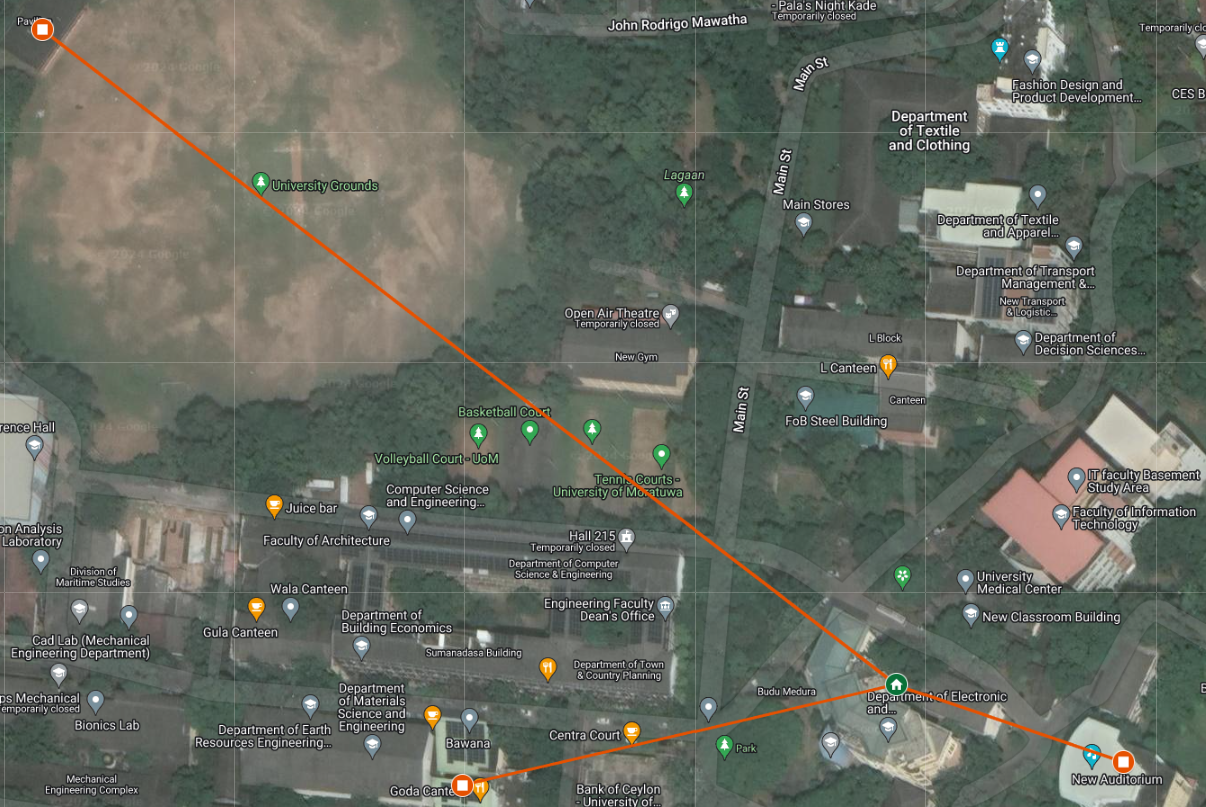
\includegraphics[width=0.8\linewidth]{images/campus test 1.png}
    \caption{Evaluation of single hop}
    \label{fig:single-hop-sim}
\end{figure}

\newpage
\subsubsection{Marine drive testing}

\begin{table}[ht!]
\begin{tabular}{|c|c|c|}
\hline
\textbf{SF} & \textbf{TX Power} & \textbf{Reception Status}                                                    \\ \hline
7           & 10dBm             & No reception                                                                 \\ \hline
8  & 10dBm & \begin{tabular}[c]{@{}c@{}}No reception (Was able \\ to detect channel activates)\end{tabular} \\ \hline
9           & 10dBm             & \begin{tabular}[c]{@{}c@{}}Had reception \\ (No consistency)\end{tabular}    \\ \hline
10 & 10dBm & \begin{tabular}[c]{@{}c@{}}Had reception (Had \\ good consistency)\end{tabular}               \\ \hline
11          & 10dBm             & \begin{tabular}[c]{@{}c@{}}Had reception \\ (Good consistency )\end{tabular} \\ \hline
12          & -                 & did not check                                                                \\ \hline
\end{tabular}
\end{table}


\begin{figure}[ht!]
    \centering
    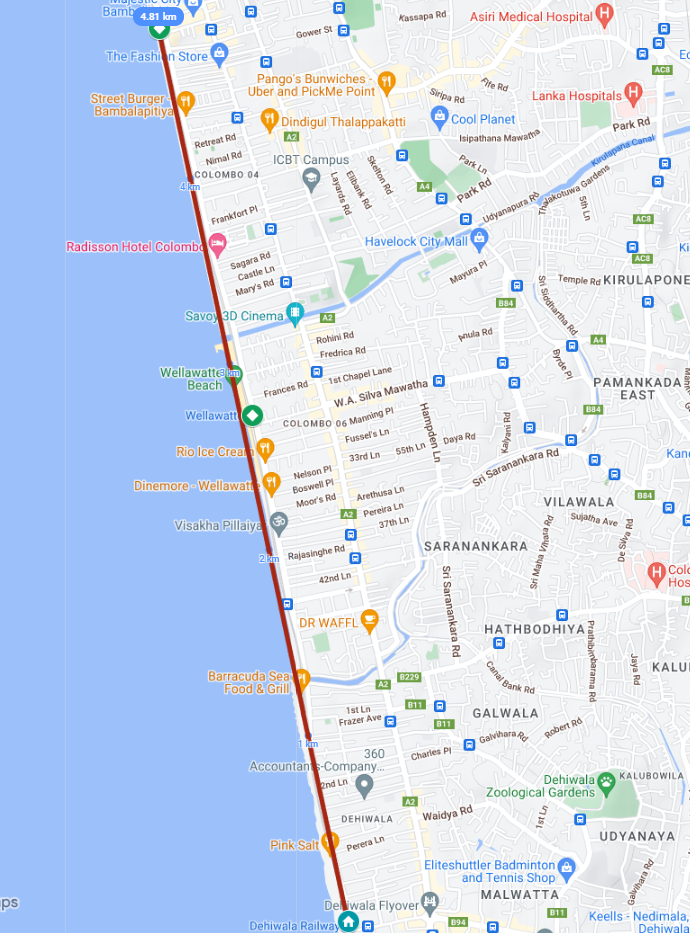
\includegraphics[width=0.5\linewidth]{images/Marinedrive.png}
    \caption{Evaluation of single hop}
    \label{fig:single-hop-sim}
\end{figure}


\newpage
\subsection{Simulation}
\label{sec:singlehop_sim}
\hspace{12pt} Initially, we examine the performance of a single-hop scenario of LoRa to gain insights into LoRa's range and \ac{ToA} characteristics within a non-free-space urban environment.

\begin{figure}[htp!]
    \centering
    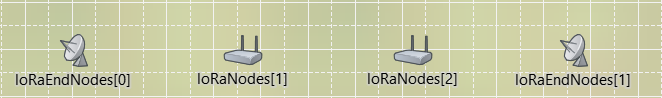
\includegraphics[width=0.8\linewidth]{images/singlehop-sim.png}
    \caption{Simulation of single hop}
    \label{fig:single-hop-sim}
\end{figure}

\begin{table}[ht!]
\centering
\resizebox{\textwidth}{!}{%
\begin{tabular}{|l|c|c|c|c|}
\hline
\multicolumn{1}{|c|}{\textbf{\begin{tabular}[c]{@{}c@{}}Spreading\\ Factor\end{tabular}}} &
  \textbf{\begin{tabular}[c]{@{}c@{}}Maximum Range\\ (m)\end{tabular}} &
  \textbf{\begin{tabular}[c]{@{}c@{}}Propagation Time\\ (seconds)\end{tabular}} &
  \textbf{\begin{tabular}[c]{@{}c@{}}Transmission Time\\ (seconds)\end{tabular}} &
  \textbf{\begin{tabular}[c]{@{}c@{}}ToA\\ (seconds)\end{tabular}} \\ \hline
SF12 & 5300 & 1.77E-05 & 1.581056 & 1.581074 \\ \hline
SF11 & 4700 & 1.57E-05 & 0.872448 & 0.872464 \\ \hline
SF10 & 4200 & 1.4E-05 & 0.436224 & 0.436238 \\ \hline
SF09 & 3500 & 1.17E-05 & 0.238592 & 0.238604 \\ \hline
SF08 & 3000 & 1E-05 & 0.129536 & 0.129546 \\ \hline
SF07 & 2600 & 8.67E-06 & 0.069888 & 0.06987 \\ \hline
\end{tabular}%
}
\caption{Comparison of single-hop performance across \ac{SF}s}
\label{tab:single-hop-sim}
\end{table}

Analysis of the \autoref{tab:single-hop-sim} reveals that the \ac{ToA} values at lower \ac{SF}s are significantly lower than those at higher \ac{SF}s.

%------------------------------------------------------------------------------------------

\newpage
\section{Evaluation of multi-hop setup}
\label{ch:multihop_evaluation}

\subsection{Experiments}
\label{sec:exp}

\subsubsection{University premises test 2}

To check the packet collision occurred by two Simultaneous relay transmitting, we checked the nature of this scenario with following setup.

\begin{figure}[ht!]
    \centering
    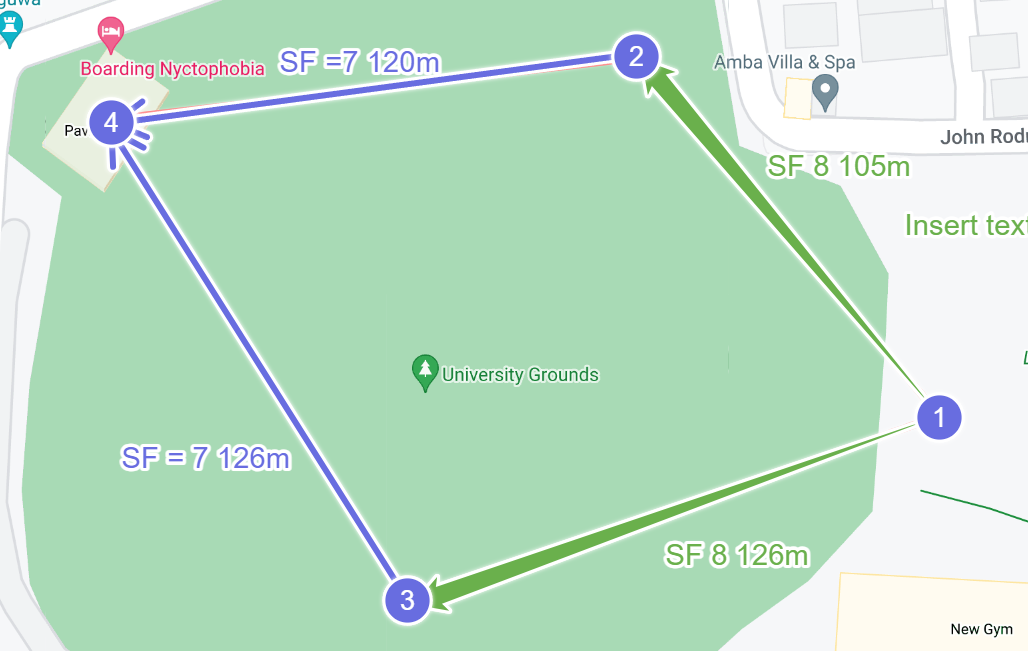
\includegraphics[width=0.8\linewidth]{images/Multirelays.png}
    \caption{Multi relay Same distance}
    \label{fig:single-hop-sim}
\end{figure}

The reception was not effected by having multiple relays transmitting packets at the same time to the same end node.


\subsection{Simulation}
\label{sec:sim}


\textbf{Scenario 01 - Achieving 5300m using lower SFs}\\

Under the aforementioned parameters, a maximum transmission range of 5800 m was determined feasible for transmitting data using SF12. Subsequently, efforts were made to achieve this distance using multihops at lower spreading factors. The detailed analysis of the results is provided below, and \autoref{tab:conclusion_1} compares the total delay reduction in this scenario, specifically highlighting the total delay reduction of lower spreading factors (SFs) compared to SF12.

\begin{table}[htp!]
\resizebox{\columnwidth}{!}{%
\begin{tabular}{|c|c|c|c|c|}
\hline
\textbf{Hop Count} &
  \textbf{\begin{tabular}[c]{@{}c@{}}Total Distance\\ (meters)\end{tabular}} &
  \textbf{\begin{tabular}[c]{@{}c@{}}Propagation Time\\ (seconds)\end{tabular}} &
  \textbf{\begin{tabular}[c]{@{}c@{}}Transmission Time\\ (seconds)\end{tabular}} &
  \multicolumn{1}{l|}{\textbf{\begin{tabular}[c]{@{}l@{}}Total Delay\\ (seconds)\end{tabular}}} \\ \hline
1 & 1800 & 6.00E-06  & 0.06988 & 0.069894 \\ \hline
2 & 3600 & 1.20E-05  & 0.13976 & 0.139788 \\ \hline
3 & 5300 & 1.767E-05 & 0.20964 & 0.209682 \\ \hline
\end{tabular}%
}
\caption{Results of 5300m multi-hop link using SF7}
\label{tab:sf_7_1}
\end{table}

\begin{table}[htp!]
\resizebox{\columnwidth}{!}{%
\begin{tabular}{|c|c|c|c|c|}
\hline
\textbf{Hop Count} &
  \textbf{\begin{tabular}[c]{@{}c@{}}Total Distance\\ (meters)\end{tabular}} &
  \textbf{\begin{tabular}[c]{@{}c@{}}Propagation Time\\ (seconds)\end{tabular}} &
  \textbf{\begin{tabular}[c]{@{}c@{}}Transmission Time\\ (seconds)\end{tabular}} &
  \multicolumn{1}{l|}{\textbf{\begin{tabular}[c]{@{}l@{}}Total Delay\\ (seconds)\end{tabular}}} \\ \hline
1 &
  2900 &
  9.67E-06 &
  0.129536 &
  0.129546 \\ \hline
2 &
  5300 &
  1.768E-05 &
  0.259072 &
  0.25909 \\ \hline
\end{tabular}%
}
\caption{Results of 5300m multi-hop link using SF8}
\label{tab:sf_8_1}
\end{table}

\begin{table}[htp!]
\resizebox{\columnwidth}{!}{%
\begin{tabular}{|c|c|c|c|l|}
\hline
\textbf{Hop Count} &
  \textbf{\begin{tabular}[c]{@{}c@{}}Total Distance\\ (meters)\end{tabular}} &
  \textbf{\begin{tabular}[c]{@{}c@{}}Propagation Time\\ (seconds)\end{tabular}} &
  \textbf{\begin{tabular}[c]{@{}c@{}}Transmission Time\\ (seconds)\end{tabular}} &
  \textbf{\begin{tabular}[c]{@{}l@{}}Total Delay\\ (seconds)\end{tabular}} \\ \hline
1 &
  2900 &
  9.67E-06 &
  0.238592 &
  0.238602 \\ \hline
2 &
  5300 &
  1.768E-05 &
  0.477184 &
  0.477202 \\ \hline
\end{tabular}%
}
\caption{Results of 5300m multi-hop link using SF9}
\label{tab:sf_9_1}
\end{table}

\begin{table}[htp!]
\resizebox{\columnwidth}{!}{%
\begin{tabular}{|c|c|c|c|c|}
\hline
\textbf{Hop Count} &
  \textbf{\begin{tabular}[c]{@{}c@{}}Total Distance\\ (meters)\end{tabular}} &
  \textbf{\begin{tabular}[c]{@{}c@{}}Propagation Time\\ (seconds)\end{tabular}} &
  \textbf{\begin{tabular}[c]{@{}c@{}}Transmission Time\\ (seconds)\end{tabular}} &
  \multicolumn{1}{l|}{\textbf{\begin{tabular}[c]{@{}l@{}}Total Delay\\ (seconds)\end{tabular}}} \\ \hline
1 &
  2900 &
  9.67E-06 &
  0.436224 &
  0.436234 \\ \hline
2 &
  5300 &
  1.768E-05 &
  0.872448 &
  0.872466 \\ \hline
\end{tabular}%
}
\caption{Results of 5300m multi-hop link using SF10}
\label{tab:sf_10_1}
\end{table}

\begin{table}[htp!]
\resizebox{\columnwidth}{!}{%
\begin{tabular}{|c|c|c|c|c|}
\hline
\textbf{Hop Count} &
  \textbf{\begin{tabular}[c]{@{}c@{}}Total Distance\\ (meters)\end{tabular}} &
  \textbf{\begin{tabular}[c]{@{}c@{}}Propagation Time\\ (seconds)\end{tabular}} &
  \textbf{\begin{tabular}[c]{@{}c@{}}Transmission Time\\ (seconds)\end{tabular}} &
  \multicolumn{1}{l|}{\textbf{\begin{tabular}[c]{@{}l@{}}Total Delay\\ (seconds)\end{tabular}}} \\ \hline
1 &
  2900 &
  9.67E-06 &
  0.872448 &
  0.872458 \\ \hline
2 &
  5300 &
  1.768E-05 &
  1.744896 &
  1.744914 \\ \hline
\end{tabular}%
}
\caption{Results of 5300m multi-hop link using SF11}
\label{tab:sf_11_1}
\end{table}

\begin{table}[htp!]
\resizebox{\columnwidth}{!}{%
\begin{tabular}{|c|c|c|c|}
\hline
\textbf{\begin{tabular}[c]{@{}c@{}}Spreading\\ Factor\end{tabular}} &
  \textbf{\begin{tabular}[c]{@{}c@{}}Minimum number of\\ hops needed\end{tabular}} &
  \textbf{\begin{tabular}[c]{@{}c@{}}Total Time Delay\\ (seconds)\end{tabular}} &
  \textbf{\begin{tabular}[c]{@{}c@{}}Time reduction compared\\ to SF12 (Seconds)\end{tabular}} \\ \hline
SF12 & 1 & 1.581074 & - \\ \hline
SF11 & 2 & 1.744914 & -0.16384 \\ \hline
SF10 & 2 & 0.872466 & 0.708608 \\ \hline
SF9  & 2 & 0.477202 & 1.103872 \\ \hline
SF8  & 2 & 0.25909 & 1.321984 \\ \hline
SF7  & 3 & 0.209682 & 1.371392 \\ \hline
\end{tabular}%
}
\caption{Performance comparison of 5300m multi hop link }
\label{tab:conclusion_1}
\end{table}

\textbf{Scenario 02 - Achieving 30km using lower SFs}\\

As our target distance is 30 km, we conducted multihop link simulations for a 30 km long link across all spreading factors. \autoref{tab:conclusion_2} provides a comparison of the performance of each spreading factor in this scenario.

\begin{table}[htp!]
\resizebox{\columnwidth}{!}{%
\begin{tabular}{|c|c|c|c|}
\hline
\textbf{\begin{tabular}[c]{@{}c@{}}Spreading\\ Factor\end{tabular}} &
  \textbf{\begin{tabular}[c]{@{}c@{}}Minimum number of\\ hops needed\end{tabular}} &
  \textbf{\begin{tabular}[c]{@{}c@{}}Total Time Delay\\ (seconds)\end{tabular}} &
  \textbf{\begin{tabular}[c]{@{}c@{}}Time reduction compared\\ to SF12 (Seconds)\end{tabular}} \\ \hline
SF12 & 6  & 9.486436 & - \\ \hline
SF11 & 7  & 6.107236 & 3.3792 \\ \hline
SF10 & 8  & 3.489892 & 5.996544 \\ \hline
SF9  & 9  & 2.147428 & 7.339008 \\ \hline
SF8  & 10 & 1.295460 & 8.190976 \\ \hline
SF7  & 12 & 0.838756 & 8.64768 \\ \hline
\end{tabular}%
}
\caption{Performance comparison of 30km multi-hop link }
\label{tab:conclusion_2}
\end{table}

\begin{figure}[htp!]
    \centering
    \begin{subfigure}{0.45\linewidth}
        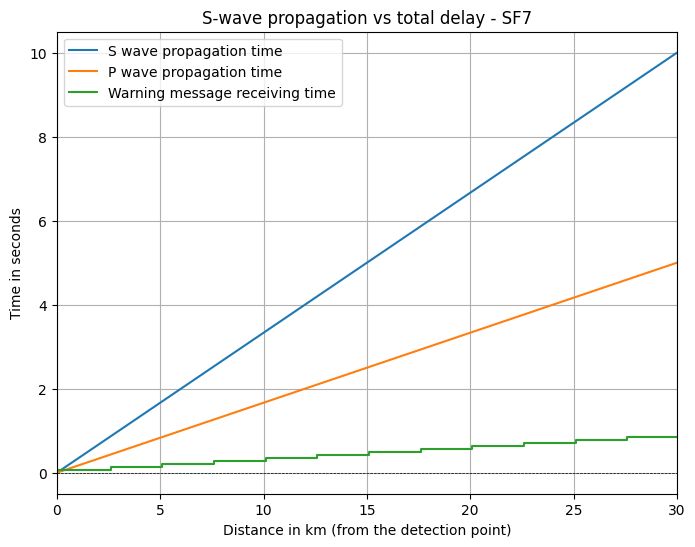
\includegraphics[width=\linewidth]{images/sf_7_30km.png}
        \caption{SF7}
    \end{subfigure}
    \hfill
    \begin{subfigure}{0.45\linewidth}
        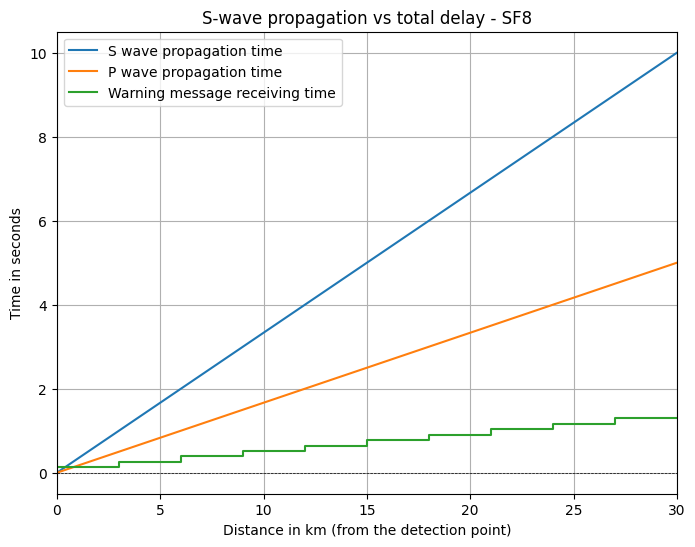
\includegraphics[width=\linewidth]{images/sf-08-30km.png}
        \caption{SF8}
    \end{subfigure}
    \\
    \begin{subfigure}{0.45\linewidth}
        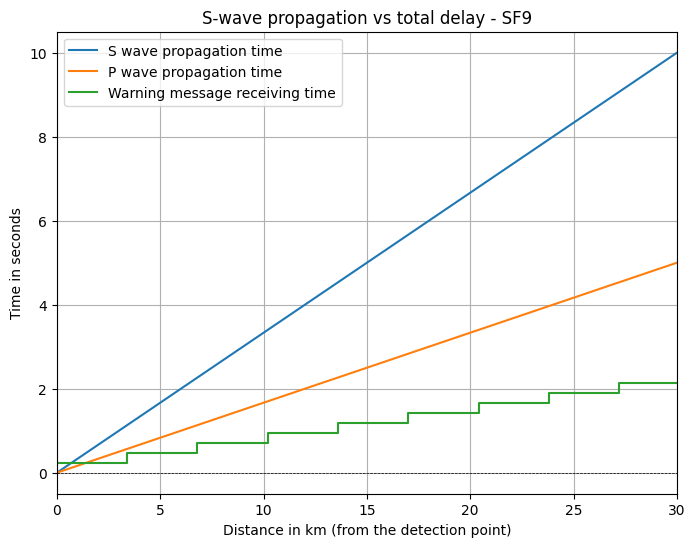
\includegraphics[width=\linewidth]{images/sf-09-30km.png}
        \caption{SF9}
    \end{subfigure}
   \hfill
    \begin{subfigure}{0.45\linewidth}
        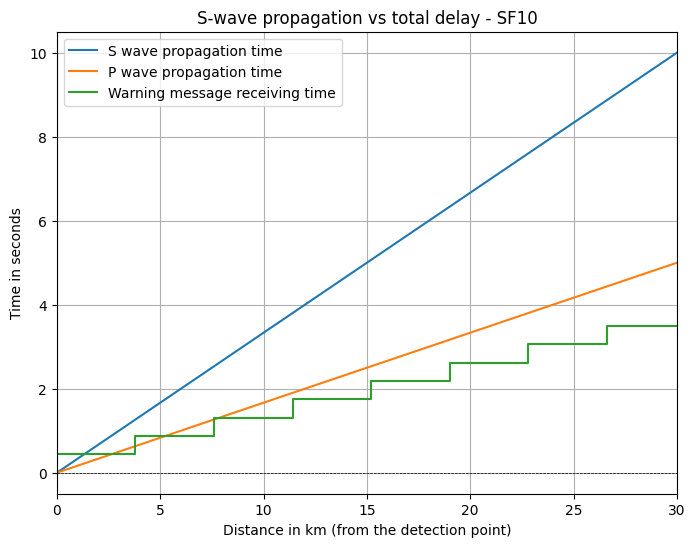
\includegraphics[width=\linewidth]{images/sf-10-30km.png}
        \caption{SF10}
    \end{subfigure}
    \\
    \begin{subfigure}{0.45\linewidth}
        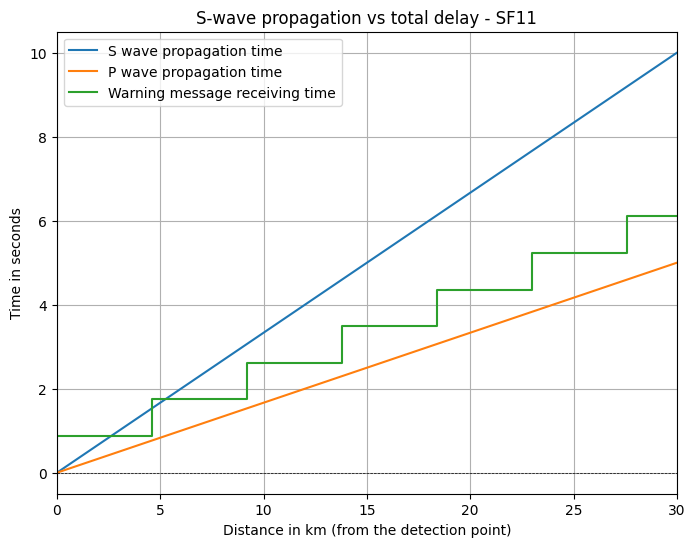
\includegraphics[width=\linewidth]{images/sf-11-30km.png}
        \caption{SF11}
    \end{subfigure}
    \hfill
    \begin{subfigure}{0.45\linewidth}
        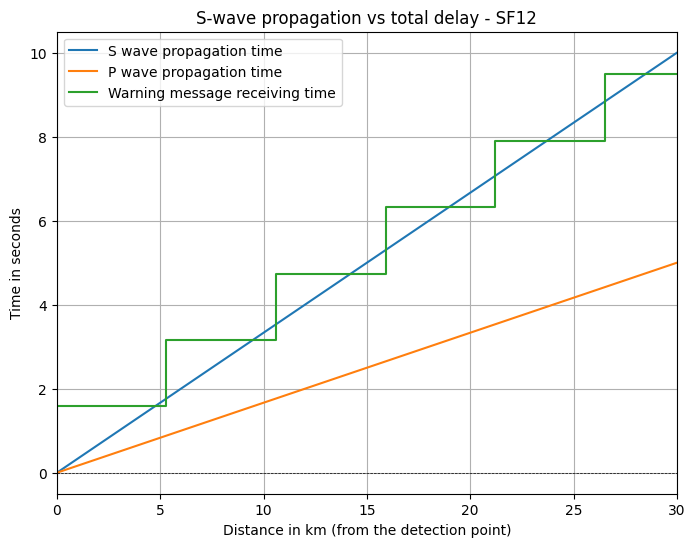
\includegraphics[width=\linewidth]{images/sf-12-30km.png}
        \caption{SF12}
    \end{subfigure}
    \caption{Seismic waves and warning message propagation time}
    \label{fig:seismic_vs_warning_message_collage}
\end{figure}

%------------------------------------------------------------------------------------------
\newpage
\section{Optimizing relays}\label{ch:relays}

Here, we tested both square and hexagonal grids using the same propagation model of Log-Normal Shadowing with identical parameters. We can see the values of unreached End nodes after 50 iterations in the square grid in \autoref{fig:unreached in square} and in the hexagonal grid in \autoref{fig:unreached in hexa}. We obtained the results presented in \autoref{tab:comparison of square and hex} after running 50 iterations with randomly changing placements of the End nodes.

\subsection{Square Grid}

Max number of Unreached nodes :- 3\\
Avg of Unreached End nodes :- 0.06$\%$

\begin{figure}[ht!]
    \centering
    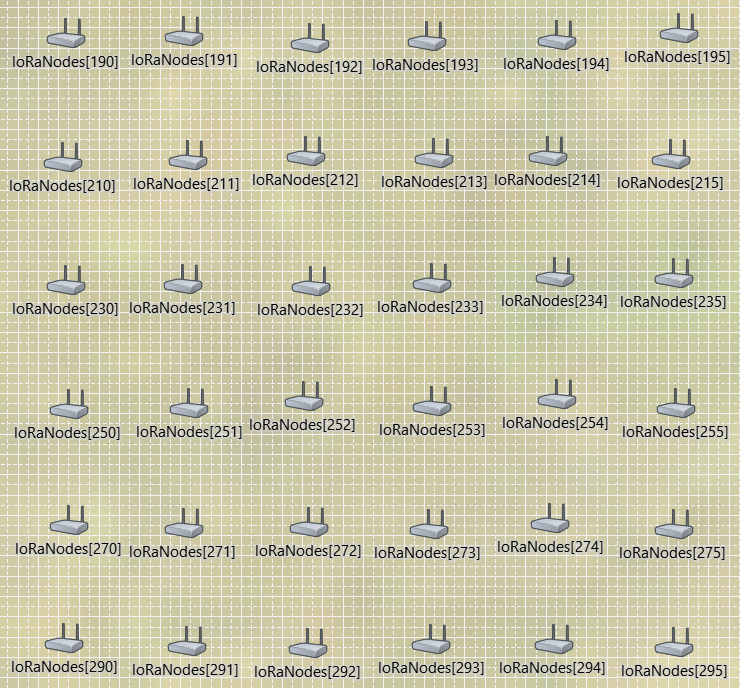
\includegraphics[scale=0.35]{images/square_grid.png}
    \caption{Relay nodes in square grid placement}
\end{figure}

\begin{figure}[ht!]
    \centering
    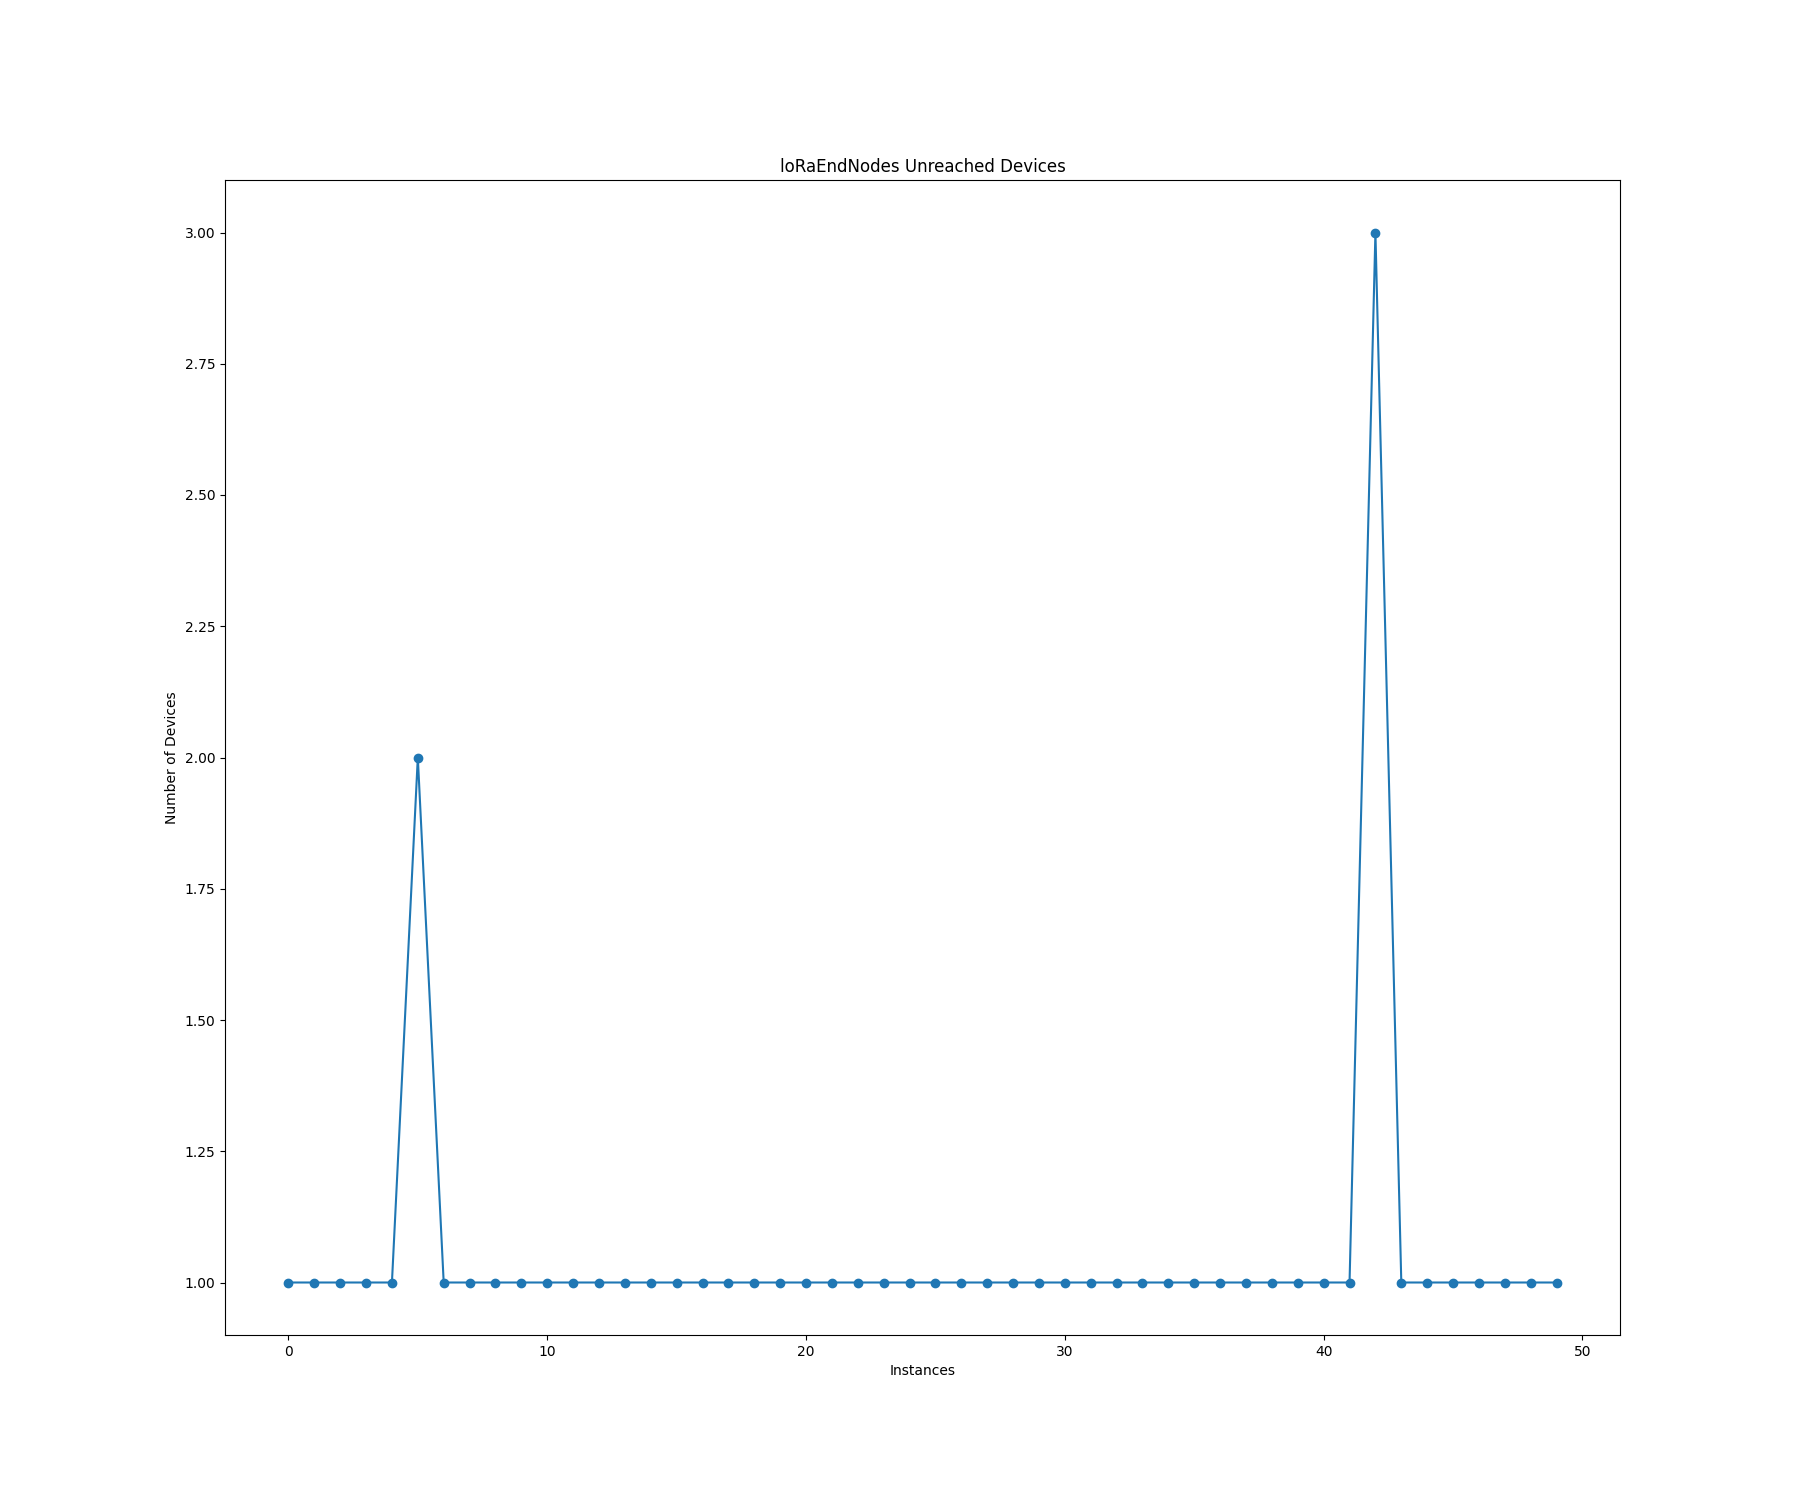
\includegraphics[scale=0.25]{images/unreached end nodes square.png}
    \caption{Unreached End nodes for 50 iterations in Square Grid }
    \label{fig:unreached in square}
\end{figure}


\newpage
\subsection{Hexagonal Grid}

Max number of Unreached nodes :- 24\\
Avg of Unreached End nodes :- 3.9$\%$

\begin{figure}[ht!]
    \centering
    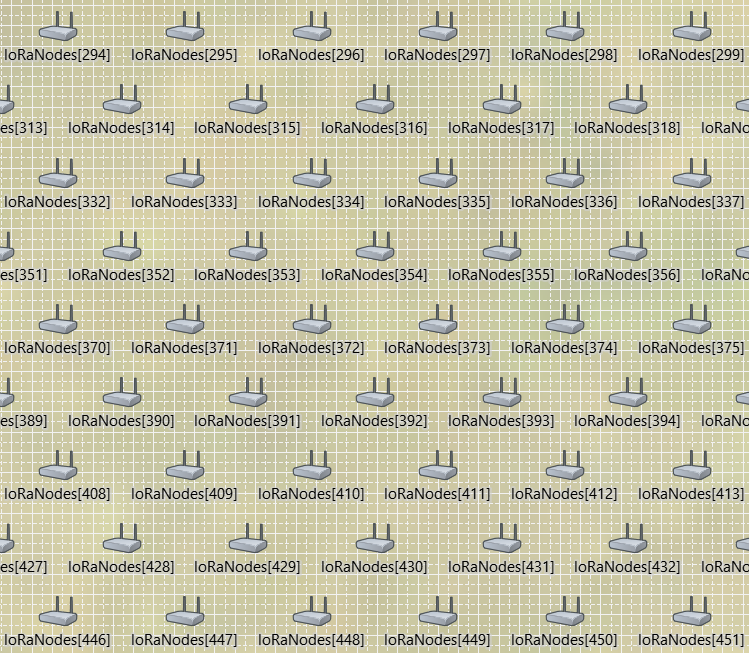
\includegraphics[scale=0.35]{images/hexa_grid.png}
    \caption{Relay nodes in hexagonal grid placement}
\end{figure}

\begin{figure}[ht!]
    \centering
    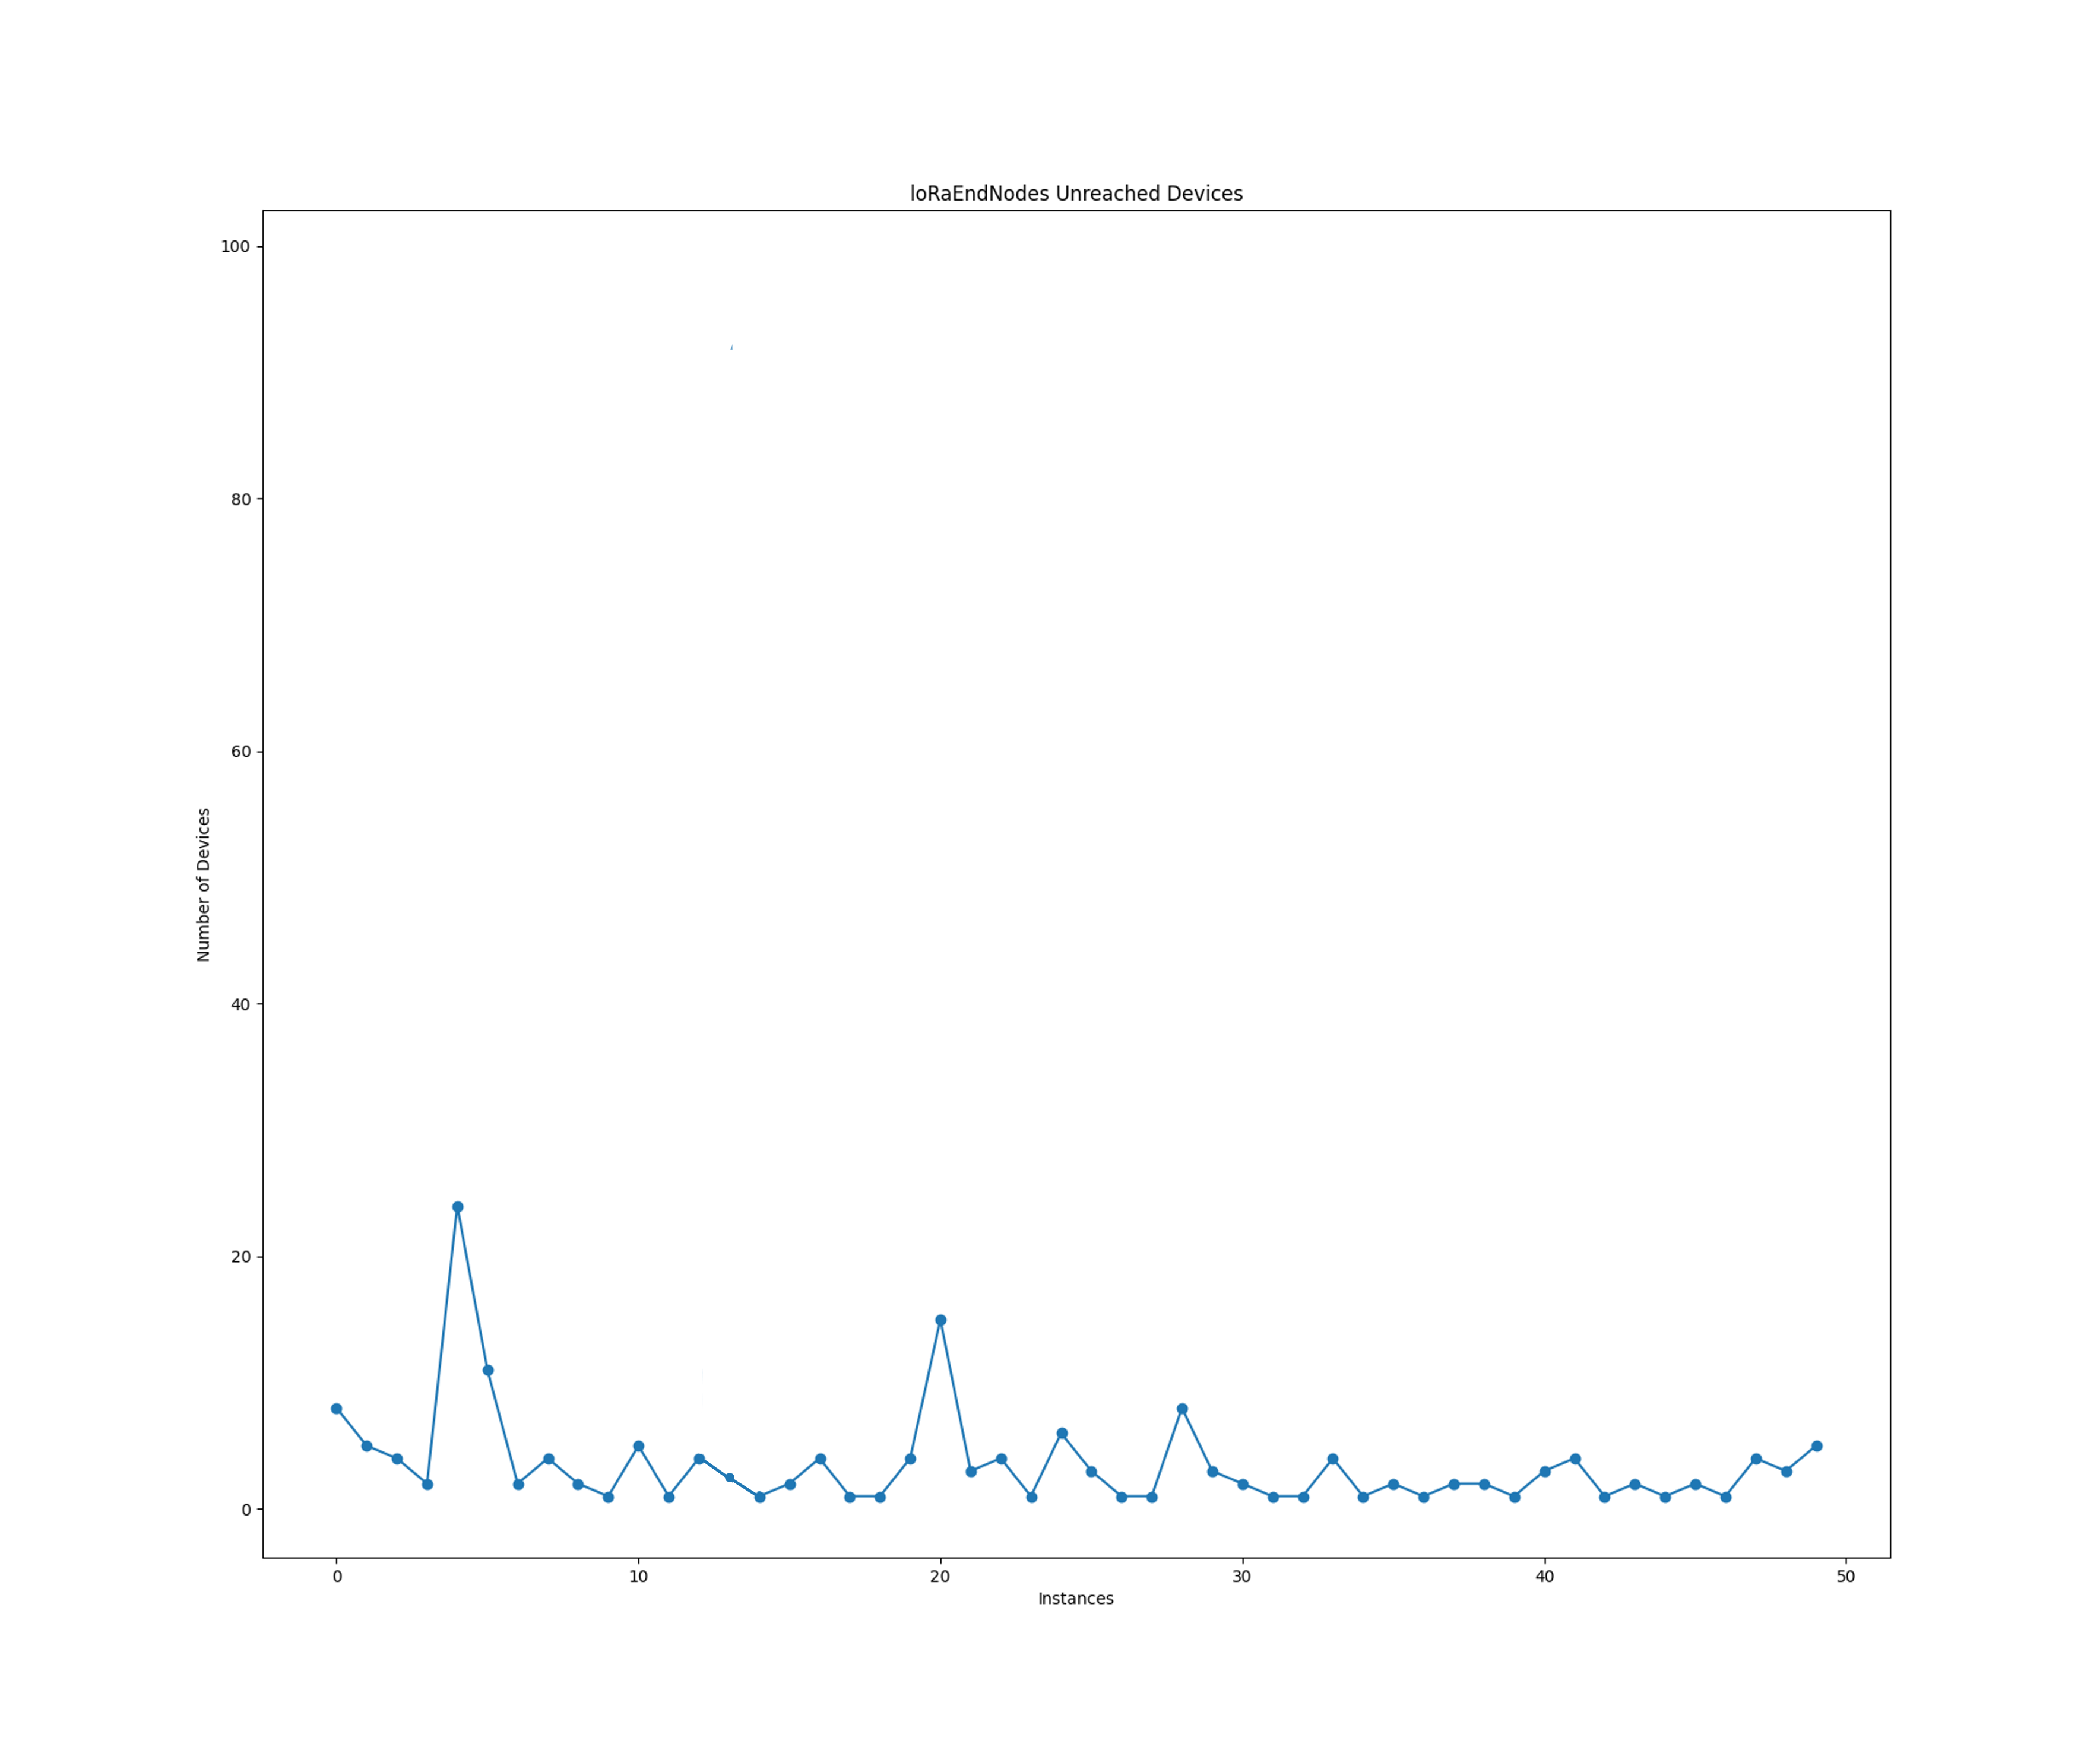
\includegraphics[scale=0.45]{images/Unreached nodes hexa.png}
    \caption{Unreached End nodes for 50 iterations in Hexa Grid }
    \label{fig:unreached in hexa}
\end{figure}



\begin{table}[ht!]
\caption{Comparison of Square and Hexa}
\begin{tabular}{|c|c|c|c|c|}
\hline
\textbf{Grid type} &
  \textbf{\begin{tabular}[c]{@{}c@{}}Total End\\ nodes\end{tabular}} &
  \textbf{\begin{tabular}[c]{@{}c@{}}Relay node\\ Density ($km^{-2}$)\end{tabular}} &
  \textbf{\begin{tabular}[c]{@{}c@{}}Avg unreached\\ End nodes\end{tabular}} &
  \textbf{\begin{tabular}[c]{@{}c@{}}Max unreached \\ reach Nodes\end{tabular}} \\ \hline
Square &
  100 &
  0.16 &
  0.06 \% &
  24 \\ \hline
Hexagonal &
  100 &
  0.17 &
  3.9 \% &
  3 \\ \hline
  
\end{tabular}
\label{tab:comparison of square and hexa}
\end{table}


\subsection{Voronoi Grid}



\begin{figure}[ht!]
    \centering
    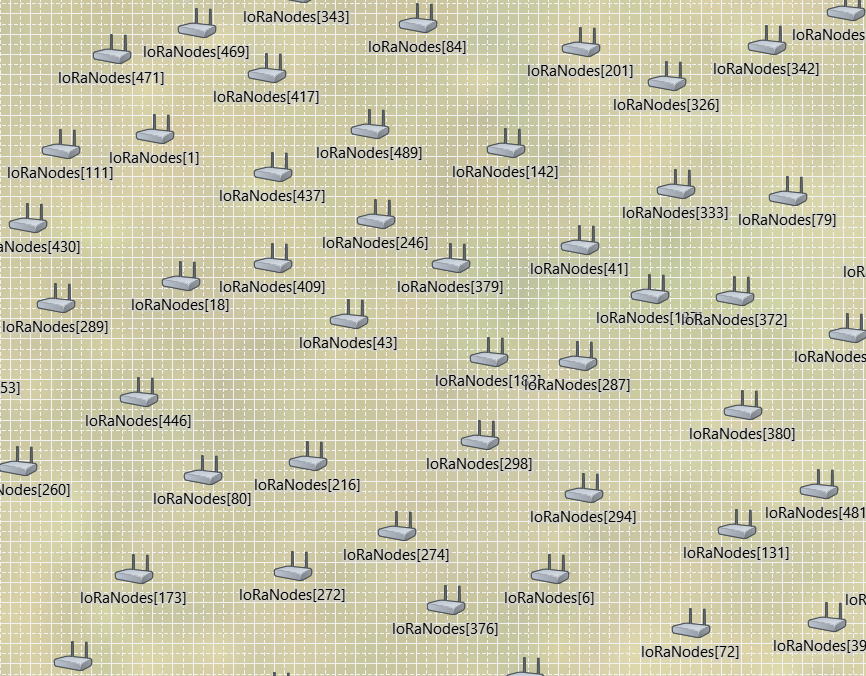
\includegraphics[scale=0.3]{images/voronoi_grid.png}
    \caption{Relay nodes in voronoi grid placement}
\end{figure}

A Voronoi diagram is a type of tessellation pattern in which a number of points scattered on a plane subdivide it into exactly n cells, each enclosing a portion of the plane that is closest to one of the points. This pattern can be found in nature, such as in cells and a giraffe's coat, as well as in architecture, art, and computer science.

We have to reject the Voronoi Grid due to the high density of Relay nodes. Additionally, random node placement is not suitable for a large city because it can result in dropped warning messages. In an earthquake warning system, stability is crucial to ensure that all packets are sent to the nodes.

Due to those reasons and comparisons, we believe that the square grid is the best architecture to set up the Relay nodes in our system. Also we able to increase the performance of the square grid adding small noise to the Relay nodes whcih are placed in the grid. The real scenario also it very practical because we can't palce the Relay nodes in exactly square grid. 

%------------------------------------------------------------------------------------------


\section{Evaluation of EEWS setup}\label{ch:eews}

We require a comprehensive architecture for EEWs, focusing on Spreading Factors and Relay Node Placement to extend warning messages beyond 30km. Our approach evaluates performance metrics while considering signal propagation and network topology. By optimizing Spreading Factors and strategically placing Relay Nodes, we aim to ensure reliable communication over extended distances. This architecture integrates technical precision with operational efficiency to enhance early earthquake warning capabilities.\\

\subsection{Simulation}
\label{sec:sim}

Our performance evaluation method involves running simulations 25 times, randomly placing End nodes within a 30km radius circular range. Through iterative interaction, the placement of End nodes changes randomly, utilizing Omnetpp's randomizing functions. This process ensures accurate assessment by reflecting the dynamic nature of the system. We conducted 25 iterations initially, but we can extend the process to more iterations.

Because of this, the system is fully crowd-driven. Therefore, our End nodes represent civilians, meaning that factors will always change. This is why we utilize totally random event iterations. Below image shows the Qtenv of the simulation with the End nodes. 


\begin{figure}[ht!]
    \centering
    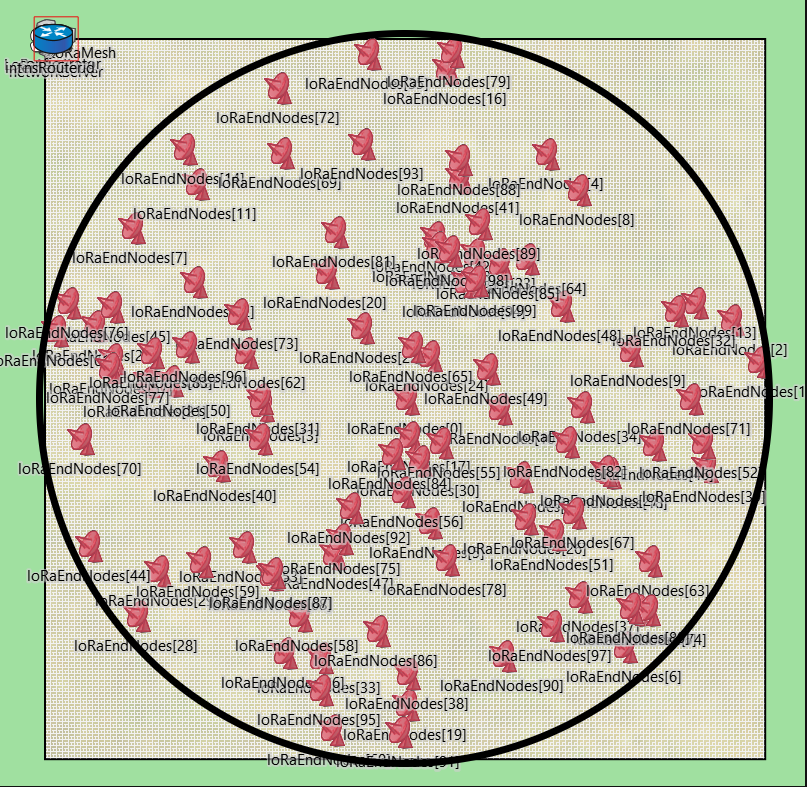
\includegraphics[scale=0.3]{images/End nodes.png}
    \caption{End nodes placement of the 30km radius circular range}
\end{figure}

The Relay nodes are placed in predetermined locations within the 30km circle. We test our simulation with different placement types: Square Grid, Hexagonal Grid, and Voronoi Grid. Based on the results, we select Square Grid as our primary Relay node placement type. Below, you can see the combination of End nodes and Relay nodes in a 60km X 60km area.



\begin{figure}
    \centering
    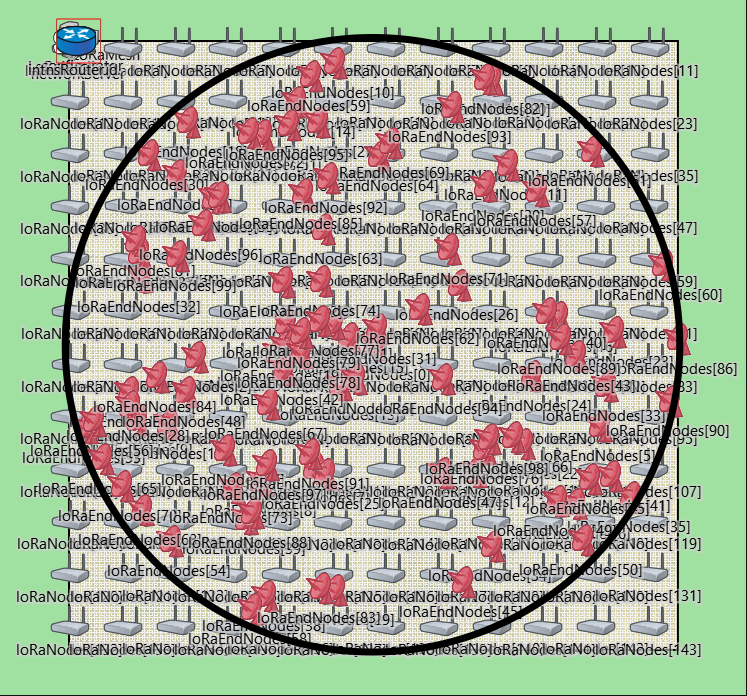
\includegraphics[width=0.6\linewidth]{images/Relays.png}
    \caption{End nodes and Relay nodes in 60km X 60km area}
    \label{fig:enter-label}
\end{figure}

We can increase the number of End nodes within the 30km radius area without any problem. However, increasing the number of Relay nodes can lead to collisions of warning message packets.

%------------------------------------------------------------------------------------------
\subsection{Simulation Results}
\label{ch:system}

Here, we mainly evaluated the performance of the spreading factors when using the best relay node placement, the Square Grid. Additionally, we improved the grid's performance by adding $\pm{100m}$ noise to the relay nodes placed in the 60km x 60km area. This adjustment significantly reduces collisions when packets are broadcasted in the grid.


\begin{figure}[ht!]
    \centering
    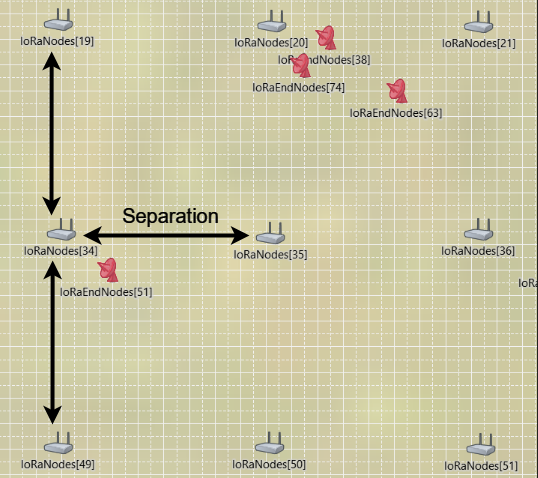
\includegraphics[width=0.6\linewidth]{images/Separation.png}
    \caption{Separation of Relay nodes}
    \label{fig:enter-label}
\end{figure}

\newpage
We use the common propagation model to evaluate the spreading factors. Our choose propagation model is Log Normal Shadowing model. So, we put the parameters to that equation of that model in OMNet++ simulation. \\

\noindent Propagation model: Log normal shadowing ($d_0=190$m, $\sigma=3.5$, $\gamma=3.3$, $PL(d_0)(dB)=96$)



\begin{table}[ht!]
\caption{Relay nodes density vs Spreading Factors}
\begin{tabular}{|c|c|c|c|c|}
\hline
\textbf{\begin{tabular}[c]{@{}c@{}}Spreading \\ Factor\end{tabular}} &
  \textbf{\begin{tabular}[c]{@{}c@{}}Separation (m) \\ $\pm{100m}$\end{tabular}} &
  \textbf{\begin{tabular}[c]{@{}c@{}}Number of \\ End nodes\end{tabular}} &
  \textbf{\begin{tabular}[c]{@{}c@{}}Number of \\ Relay nodes\end{tabular}} &
  \textbf{\begin{tabular}[c]{@{}c@{}}Relay node \\ coverage ($km^2$ )\end{tabular}} \\ \hline
7  & 2300 & 100 & 676 & 5.325 \\ \hline
8  & 3200 & 100 & 361 & 9.975 \\ \hline
9  & 4100 & 100 & 225 & 16    \\ \hline
10 & 5200 & 100 & 144 & 25    \\ \hline
11 & 6400 & 100 & 100 & 36    \\ \hline
12 & 7800 & 100 & 64  & 56.25 \\ \hline
\end{tabular}
\end{table}

According to the above table, we should remove \ac{SF} 7 due to its high Relay node density, which would increase our system costs. However, our system aims to be a low-cost Early Earthquake Warning system. Moreover, high Relay node density may lead to warning message collisions.\\

After conducting 25 iterations of the simulation, we can extract the results using OMNeT++. We utilize the batch simulation method to obtain the elog files, which contain every event that occurred during the simulation duration. Initially, we enable Event Log Recording in OMNeT++ and then proceed to run our batch simulation across 25 fully random iterations.

% \\\\\\\\\\\\\\\\\\\\\\\\\\\\\\\\\\\\\\\\\\\\\\\\\\\\\\

\begin{figure}[ht!]

    \centering
    \begin{subfigure}{0.45\linewidth}
        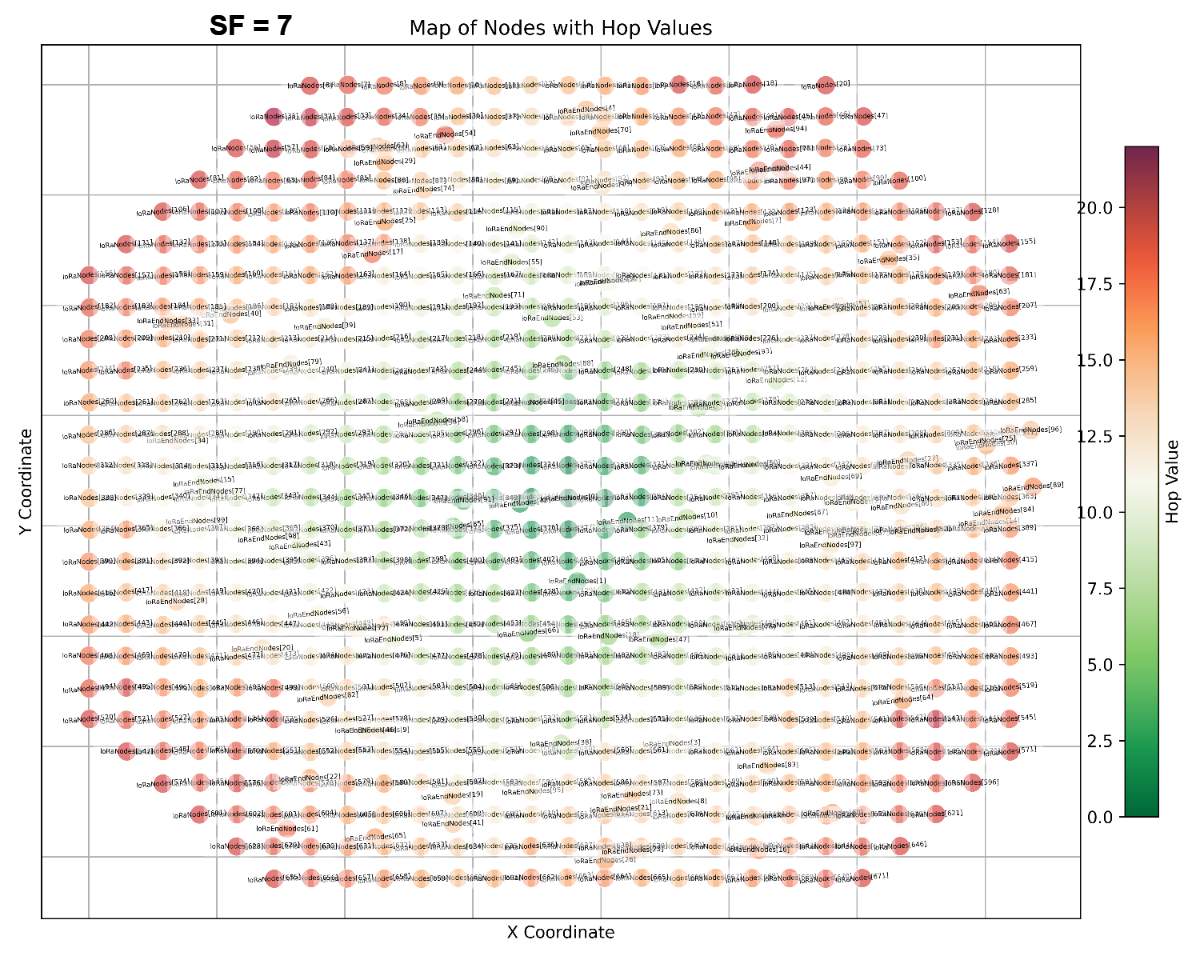
\includegraphics[width=\linewidth]{images/nodeplacement1.png}
        \caption{SF7}
    \end{subfigure}
    \hfill
    \begin{subfigure}{0.45\linewidth}
        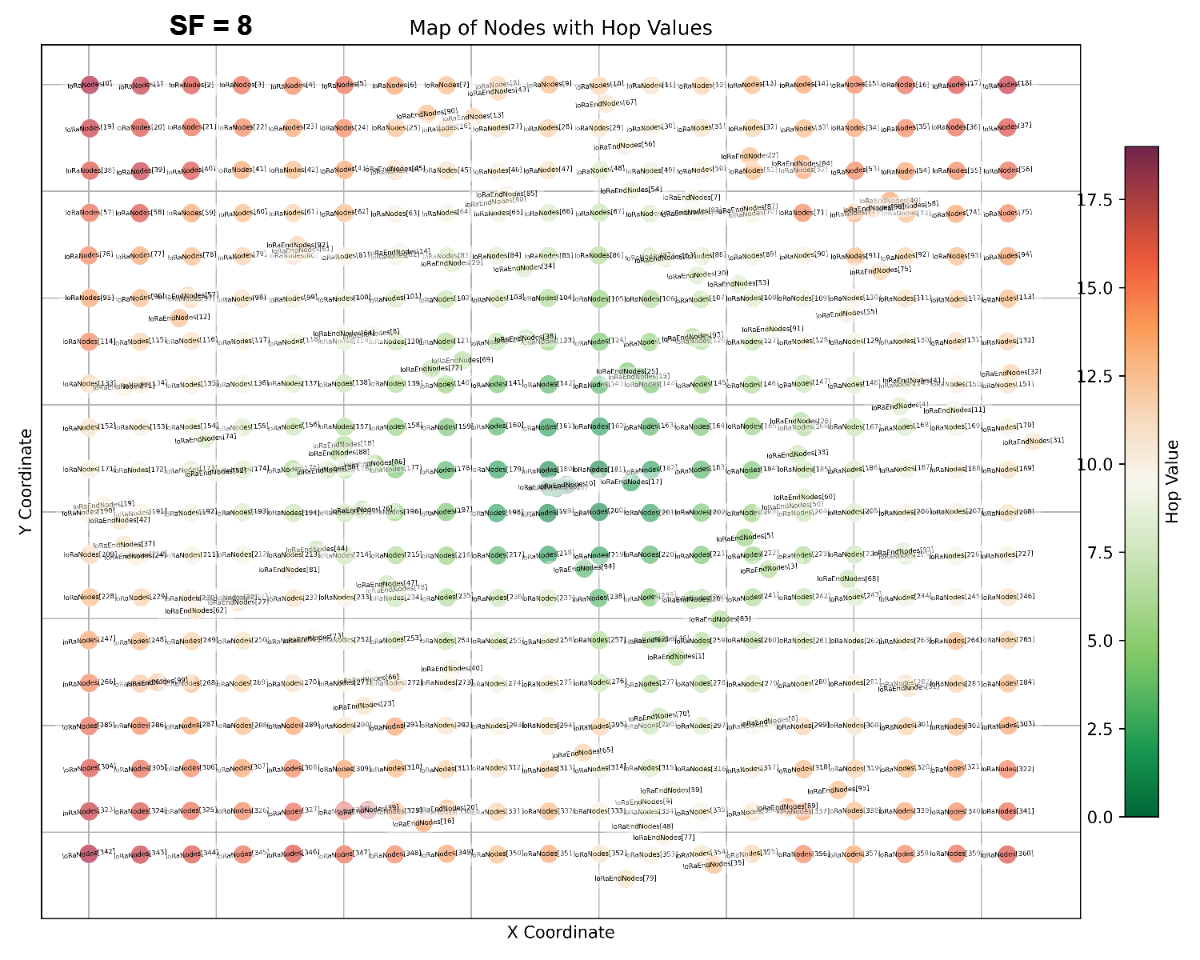
\includegraphics[width=\linewidth]{images/nodeplacement2.png}
        \caption{SF8}
    \end{subfigure}
    \\
    \begin{subfigure}{0.45\linewidth}
        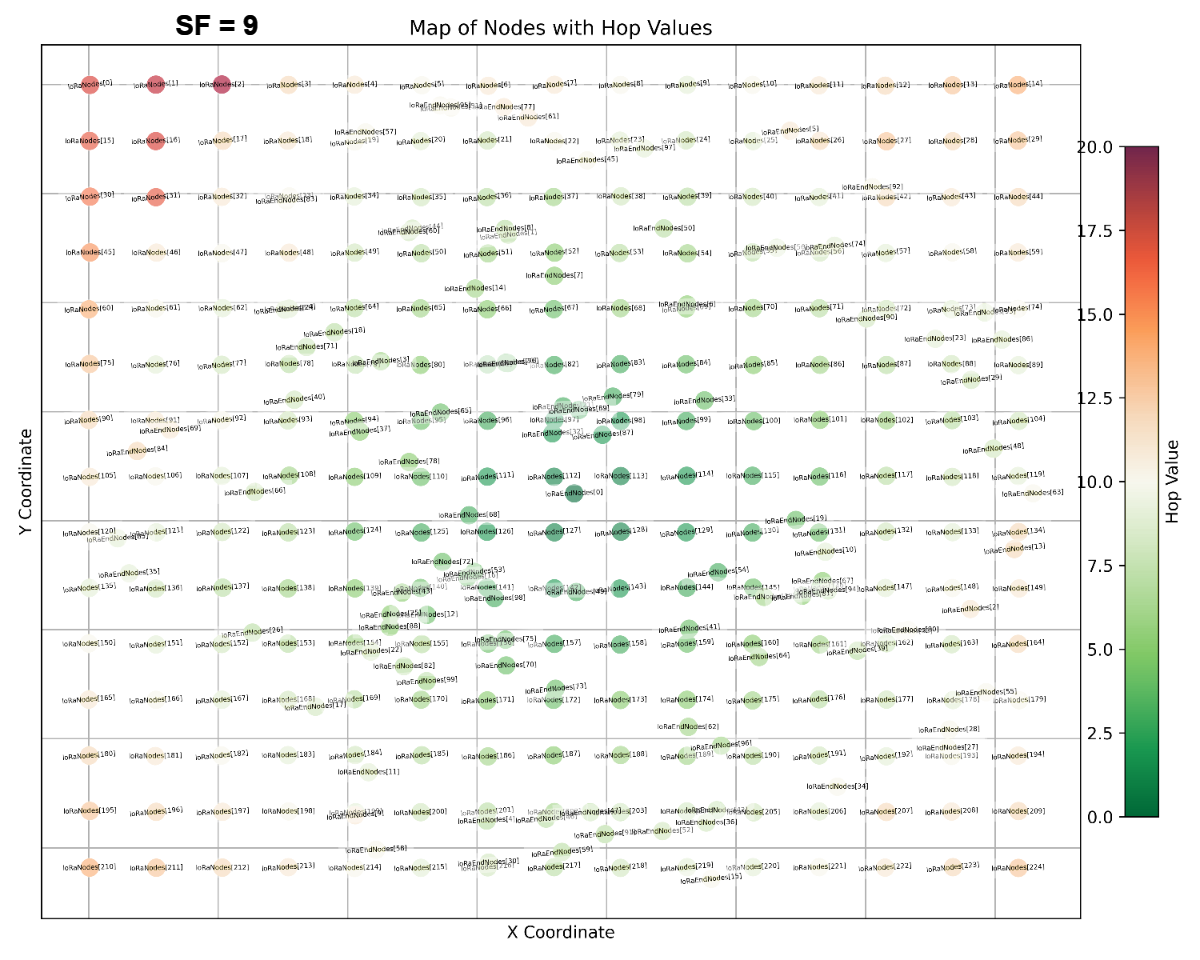
\includegraphics[width=\linewidth]{images/nodeplacement3.png}
        \caption{SF9}
    \end{subfigure}
   \hfill
    \begin{subfigure}{0.45\linewidth}
        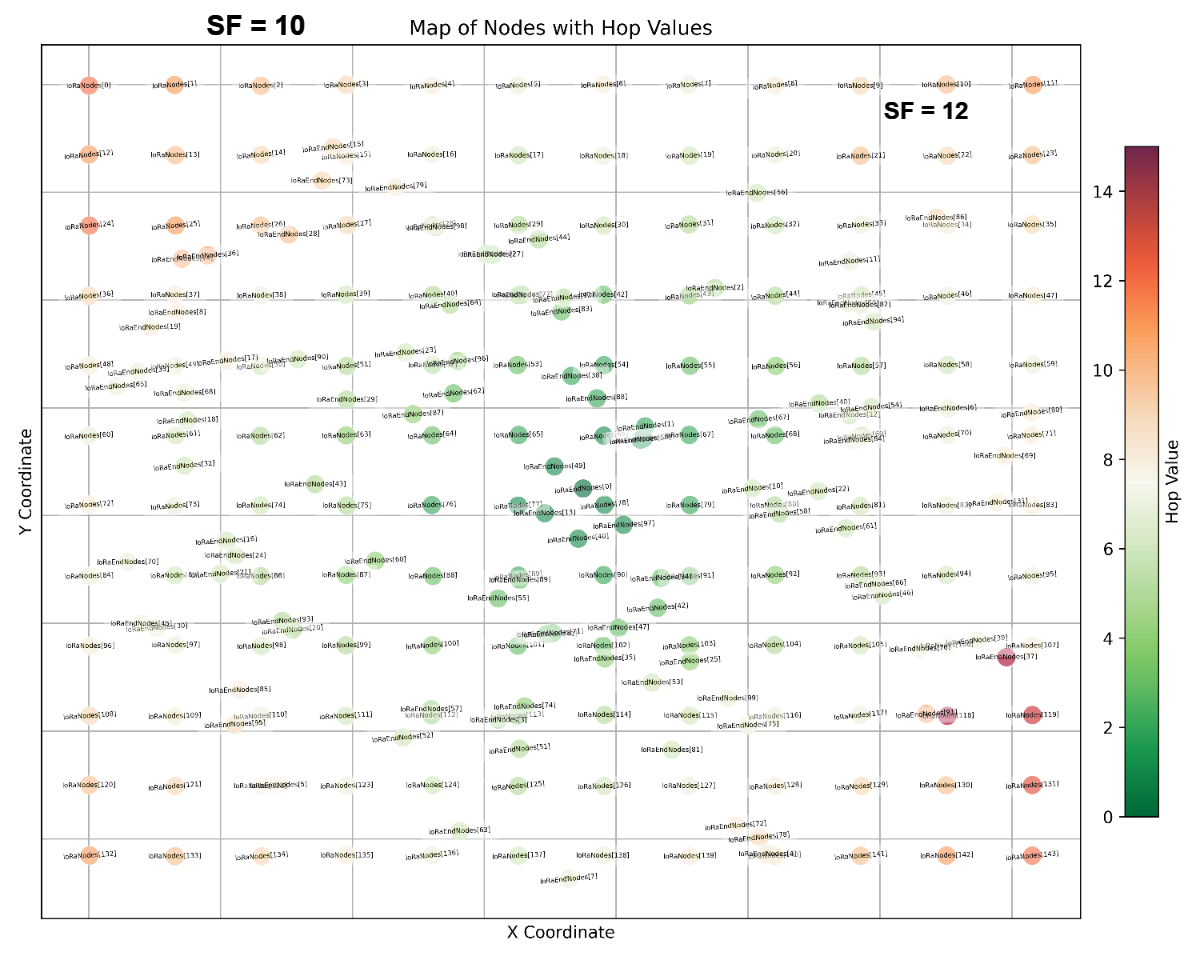
\includegraphics[width=\linewidth]{images/nodeplacement4.png}
        \caption{SF10}
    \end{subfigure}
    \\
    \begin{subfigure}{0.45\linewidth}
        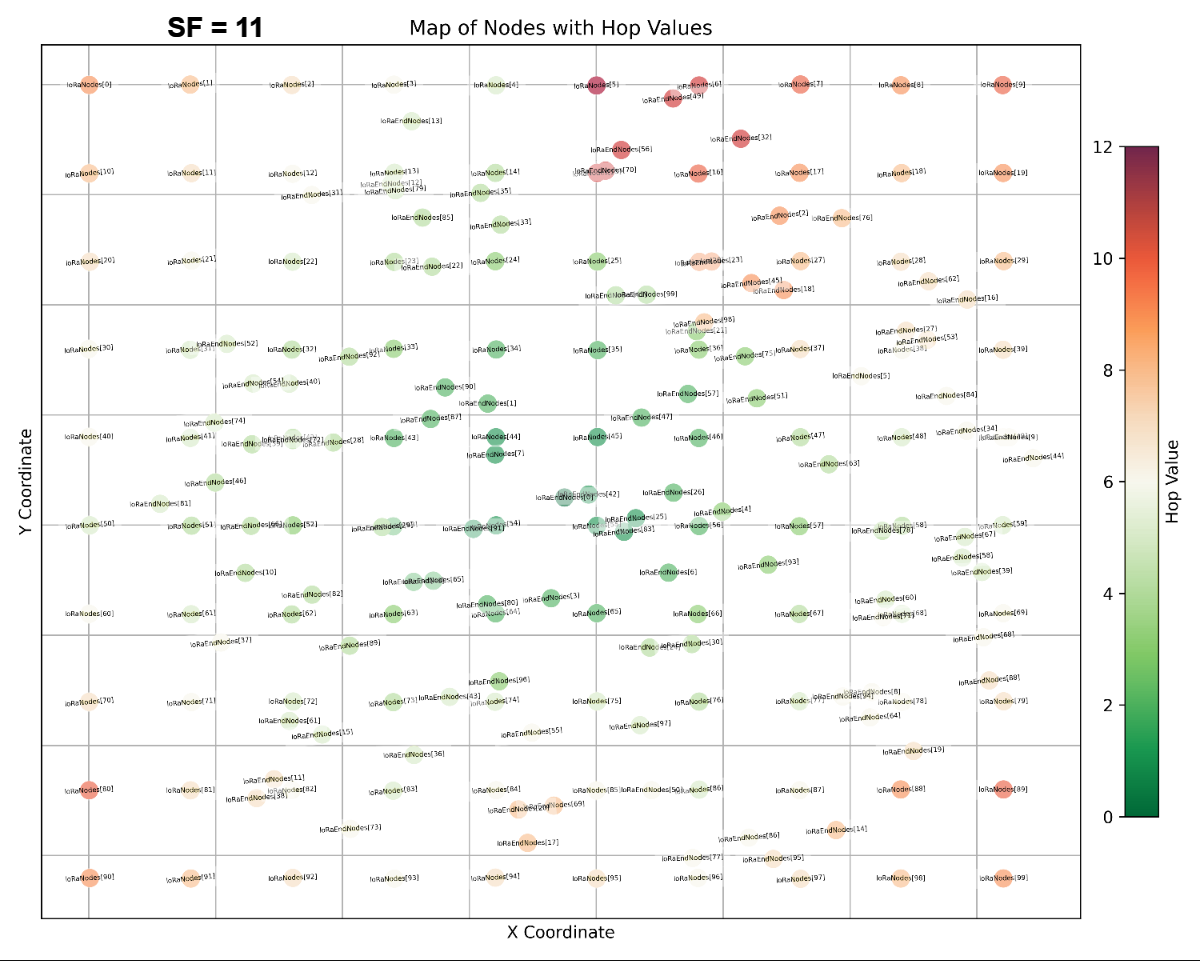
\includegraphics[width=\linewidth]{images/nodeplacement5.png}
        \caption{SF11}
    \end{subfigure}
    \hfill
    \begin{subfigure}{0.45\linewidth}
        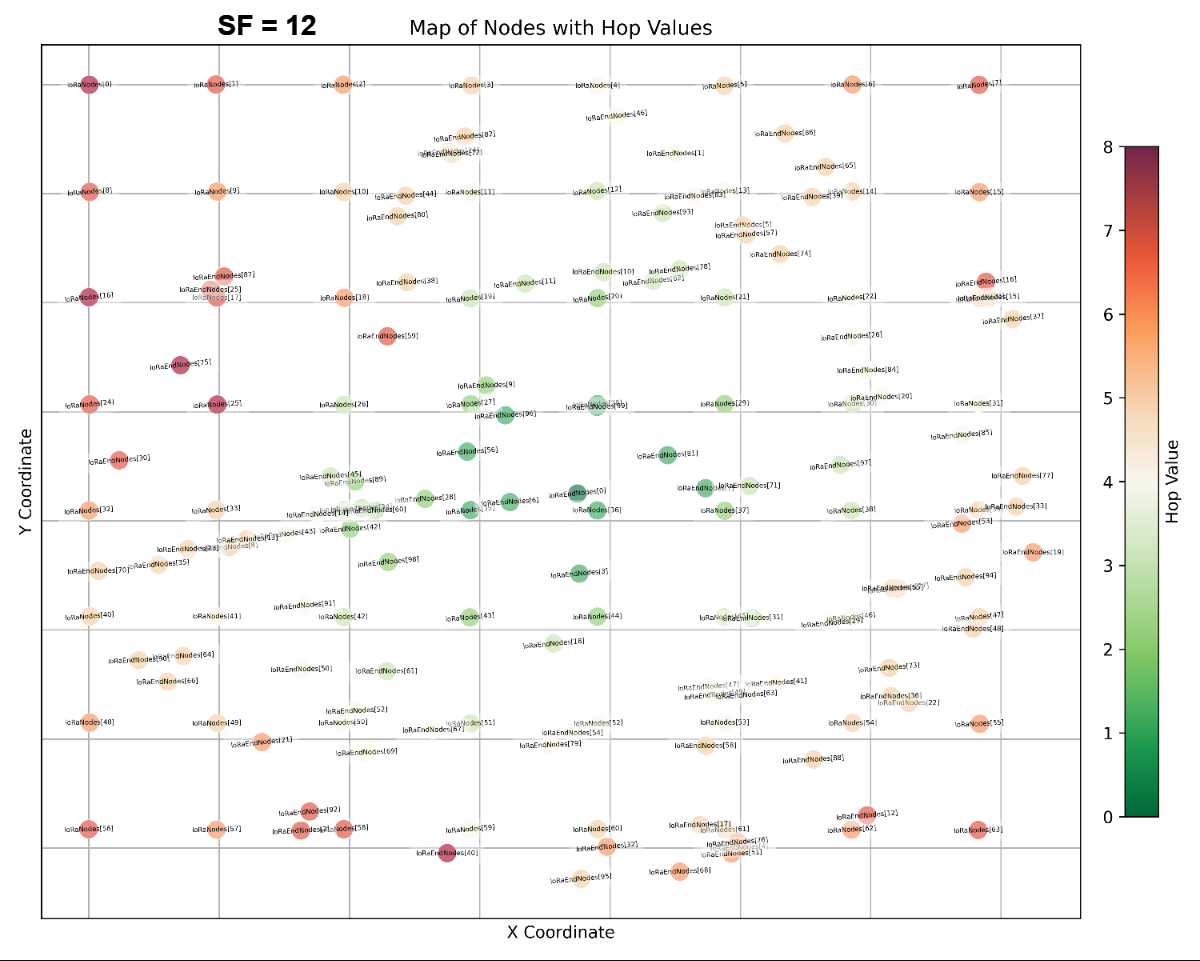
\includegraphics[width=\linewidth]{images/nodeplacement6.png}
        \caption{SF12}
    \end{subfigure}
    \caption{Node Placements vs Hop Count of Spreading Factors}
    \label{fig:nodeplacement collage}
\end{figure}

% \\\\\\\\\\\\\\\\\\\\\\\\\\\\\\\\\\\\\\\\\\\\\\\\\\\\\\
\newpage

\begin{figure}[htp!]
    \centering
    \begin{subfigure}{0.45\linewidth}
        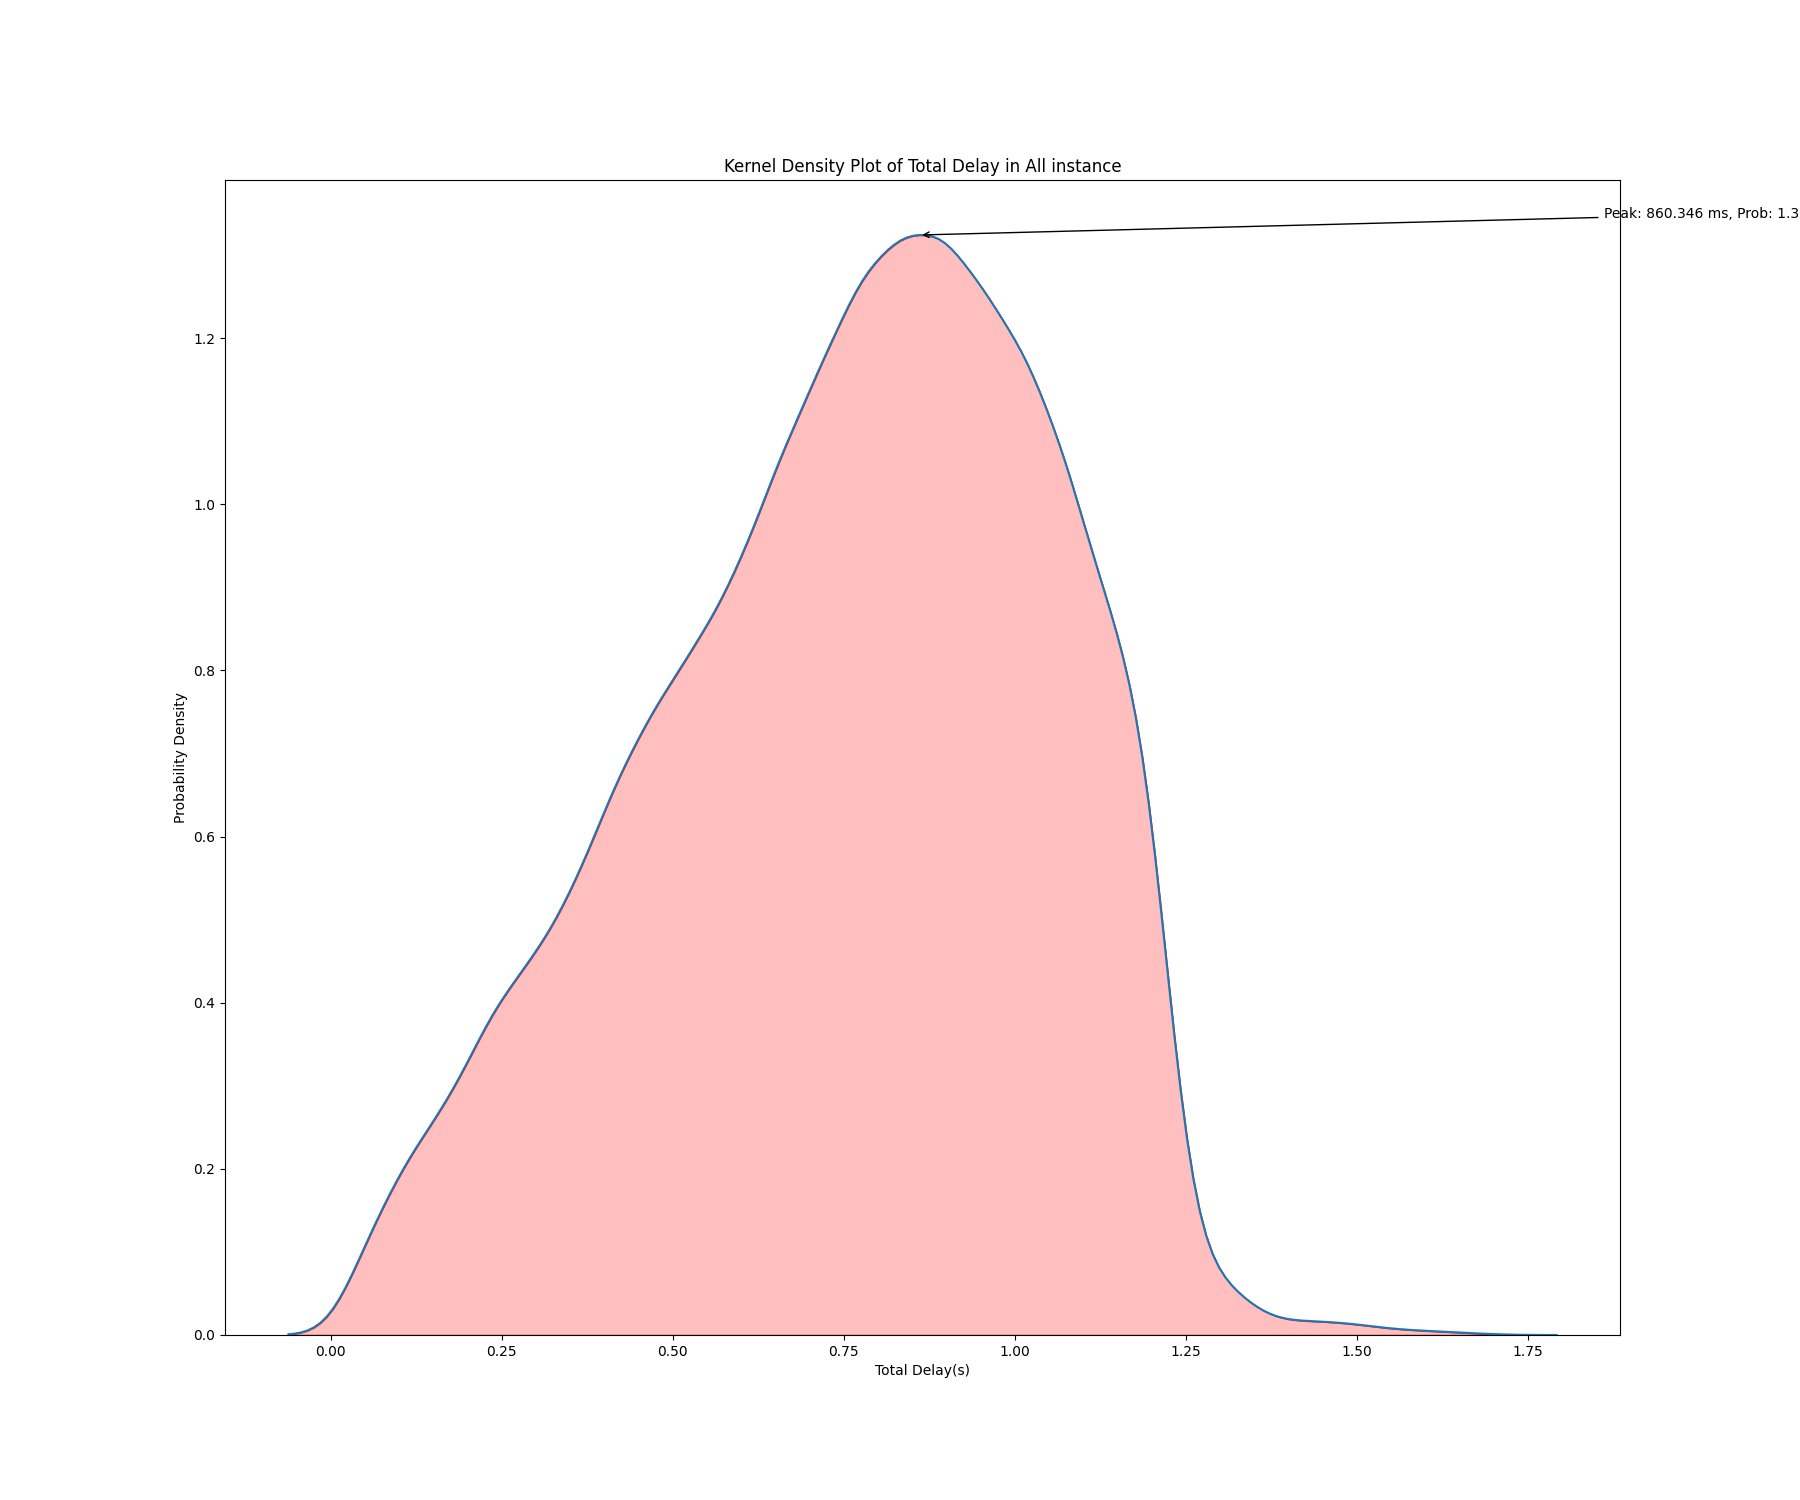
\includegraphics[width=\linewidth]{images/Total Delay density1.png}
        \caption{SF7}
    \end{subfigure}
    \hfill
    \begin{subfigure}{0.45\linewidth}
        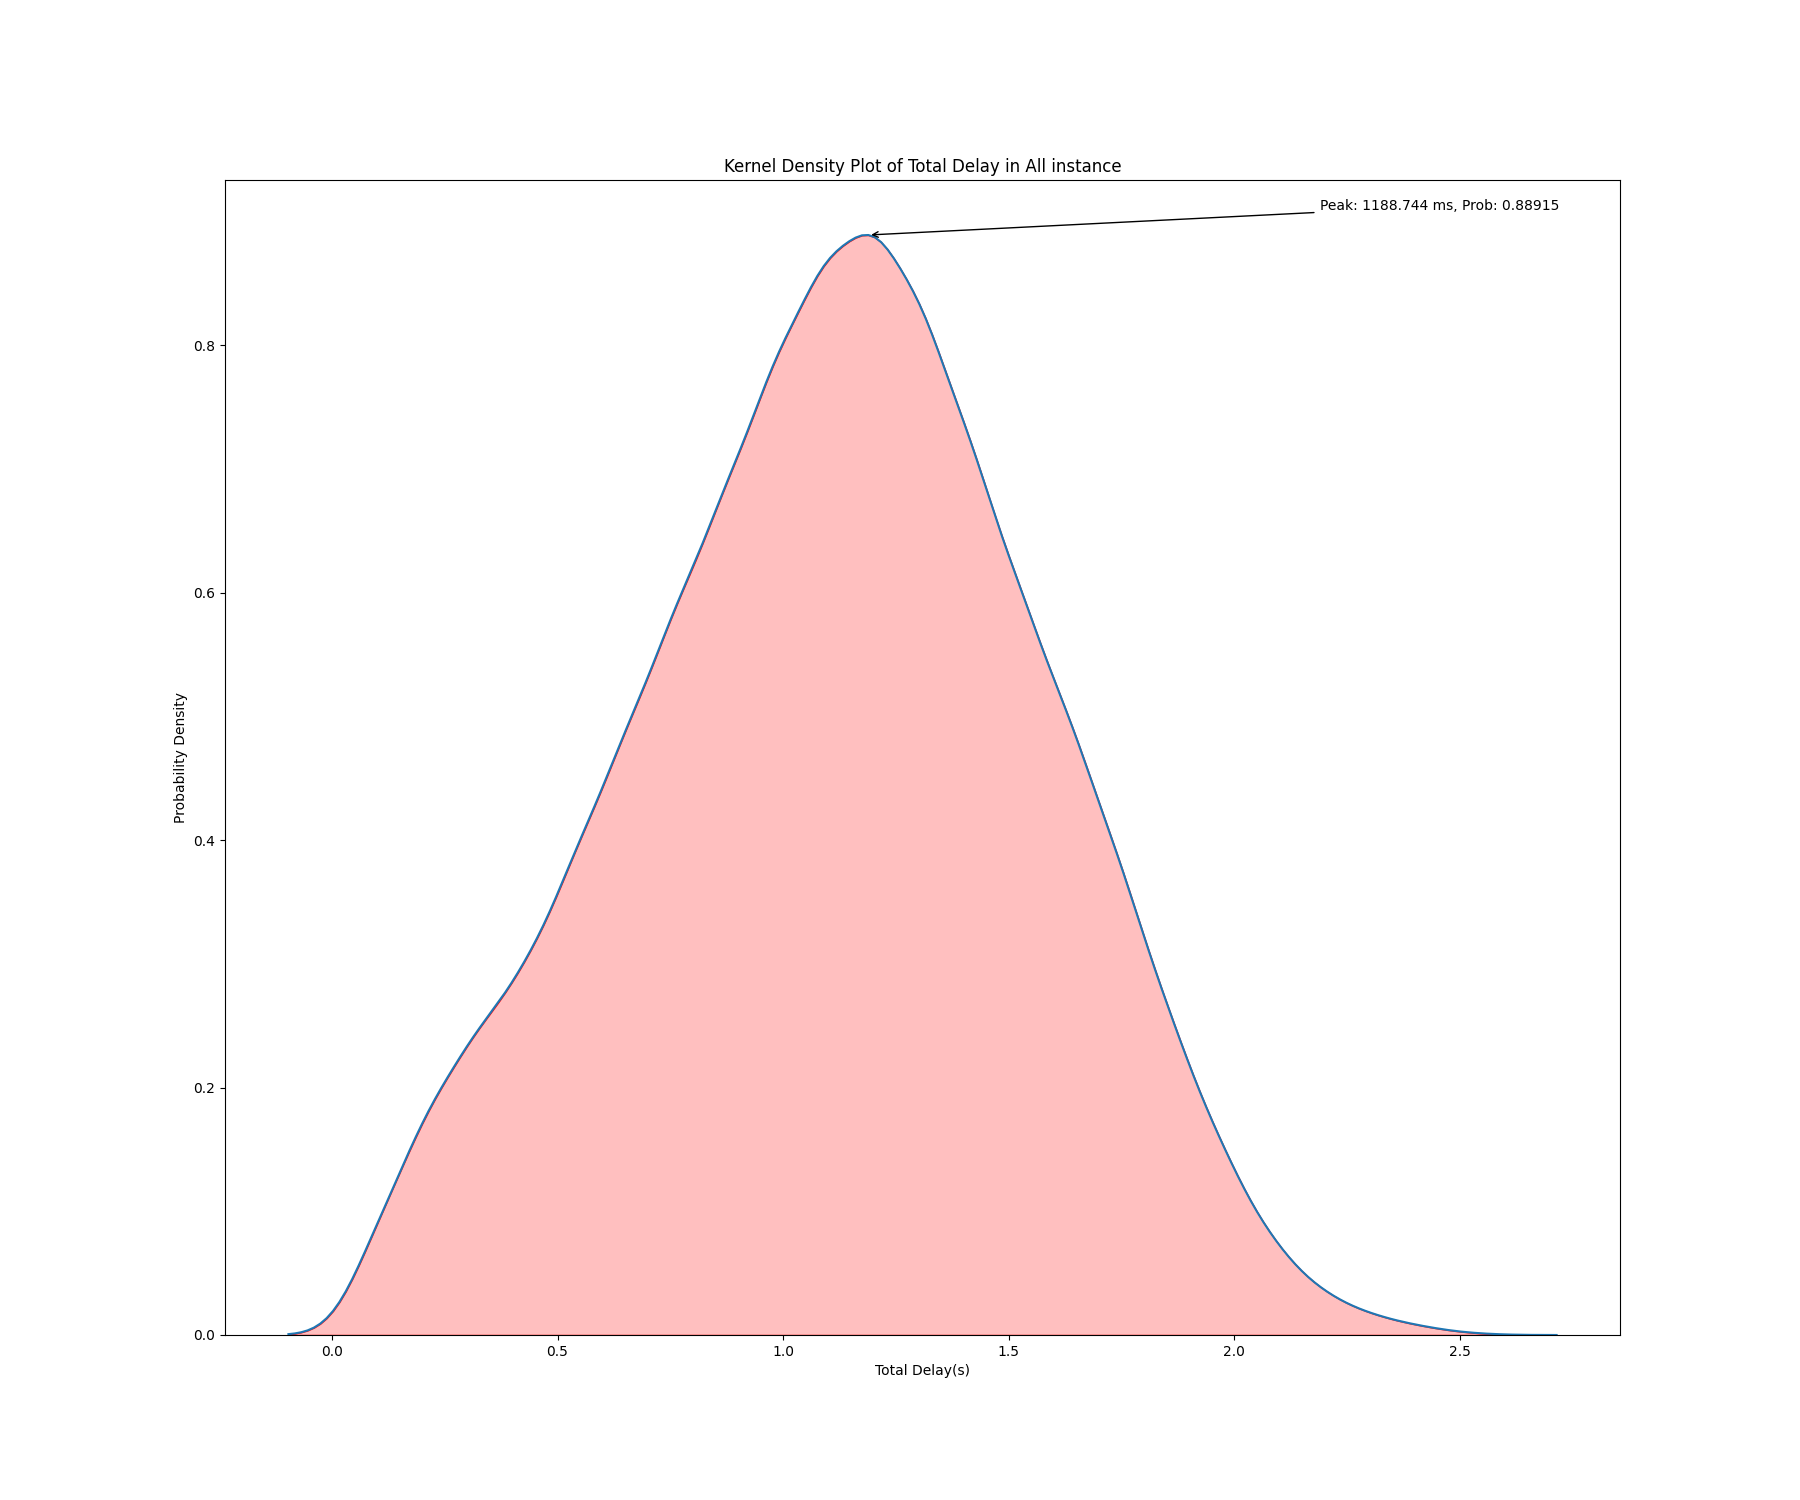
\includegraphics[width=\linewidth]{images/Total Delay density2.png}
        \caption{SF8}
    \end{subfigure}
    \\
    \begin{subfigure}{0.45\linewidth}
        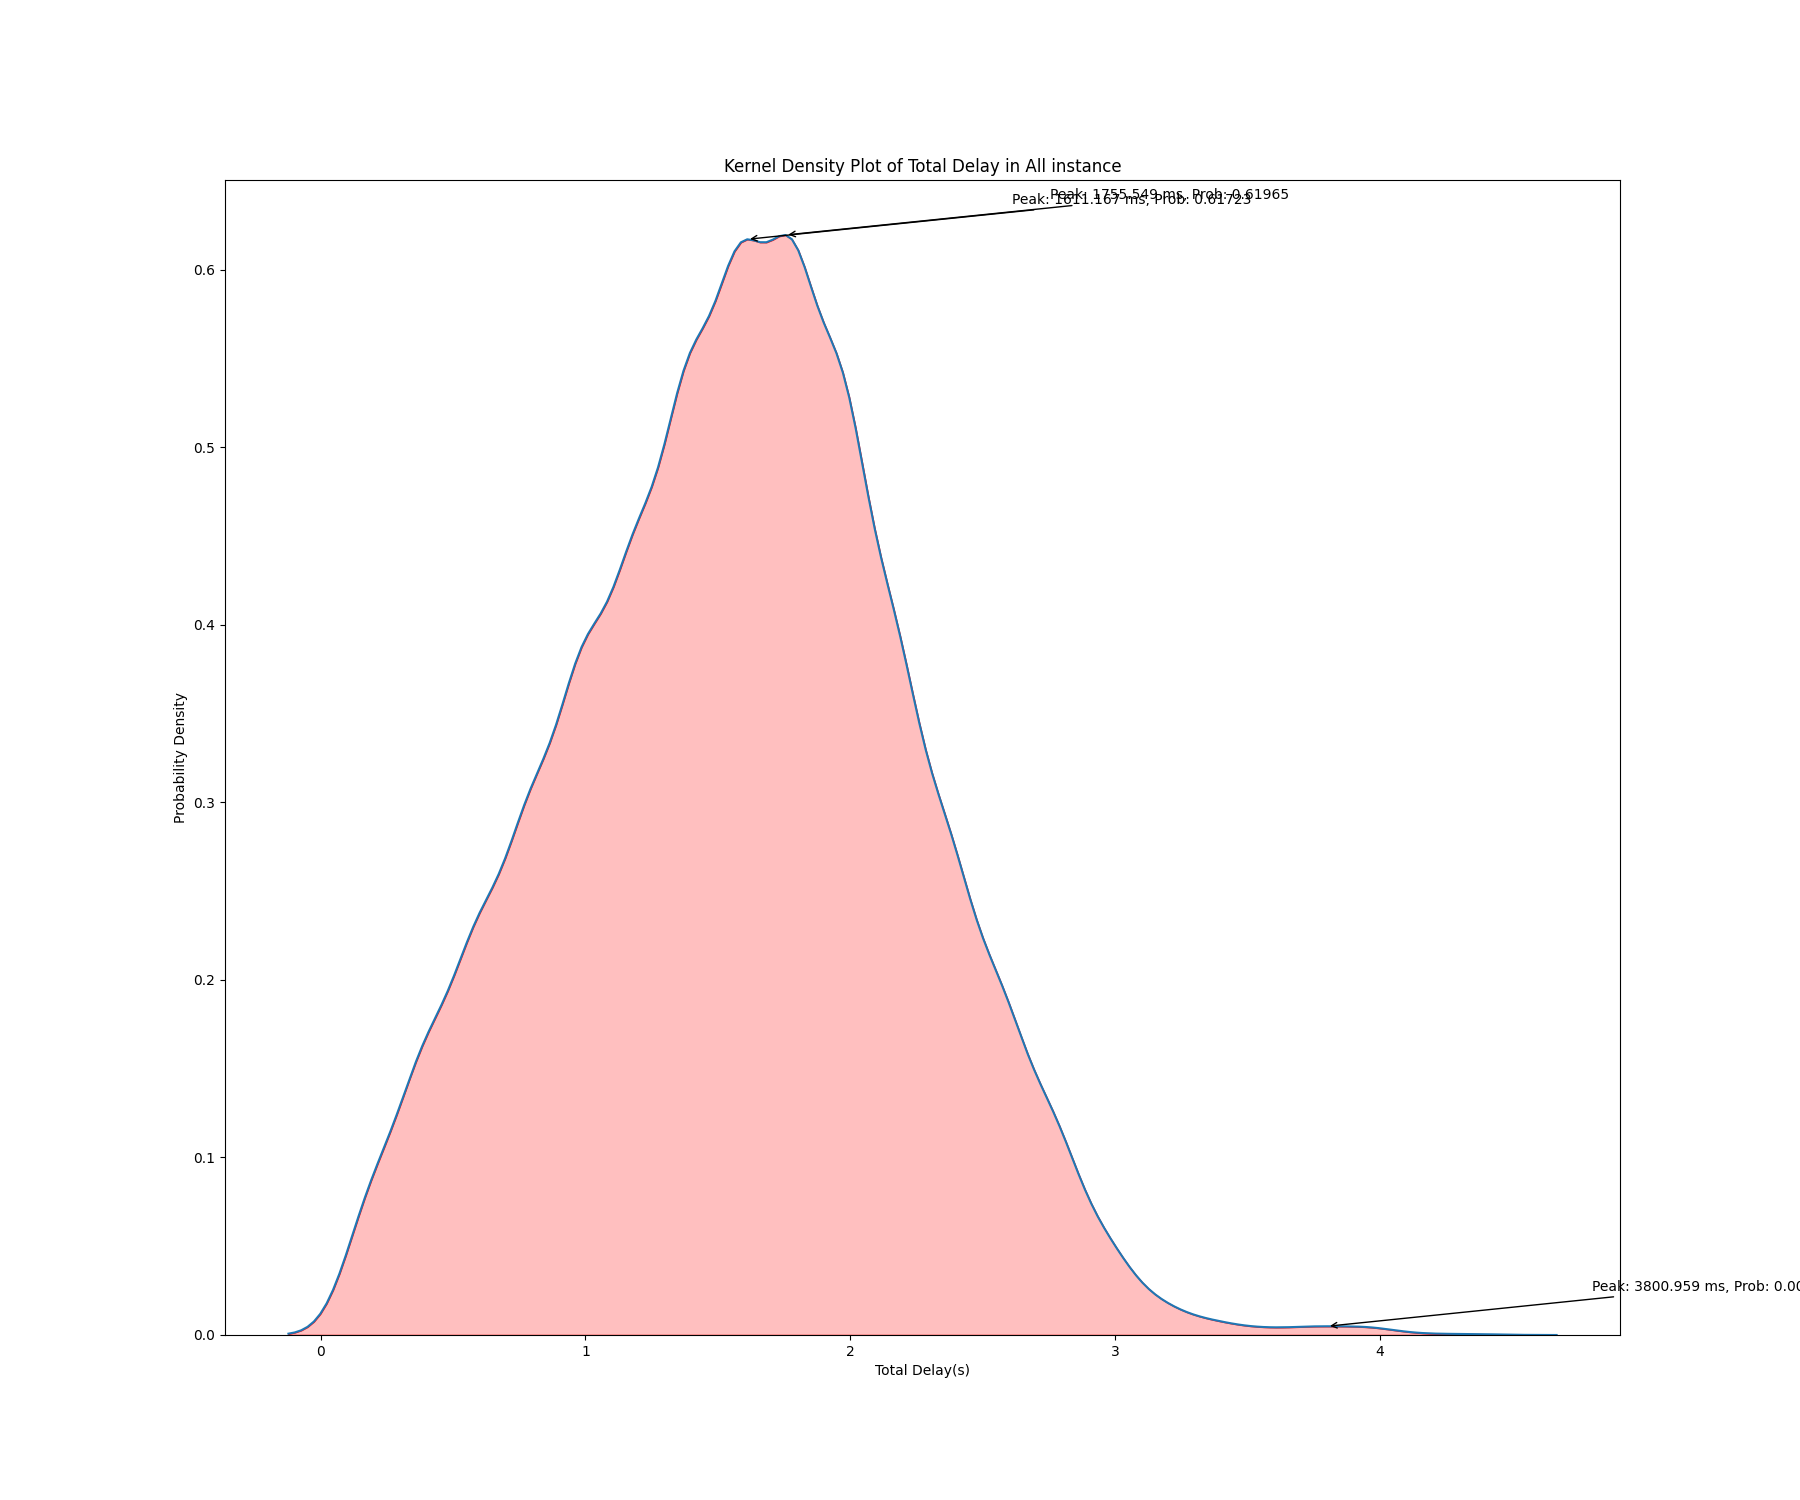
\includegraphics[width=\linewidth]{images/Total Delay density3.png}
        \caption{SF9}
    \end{subfigure}
   \hfill
    \begin{subfigure}{0.45\linewidth}
        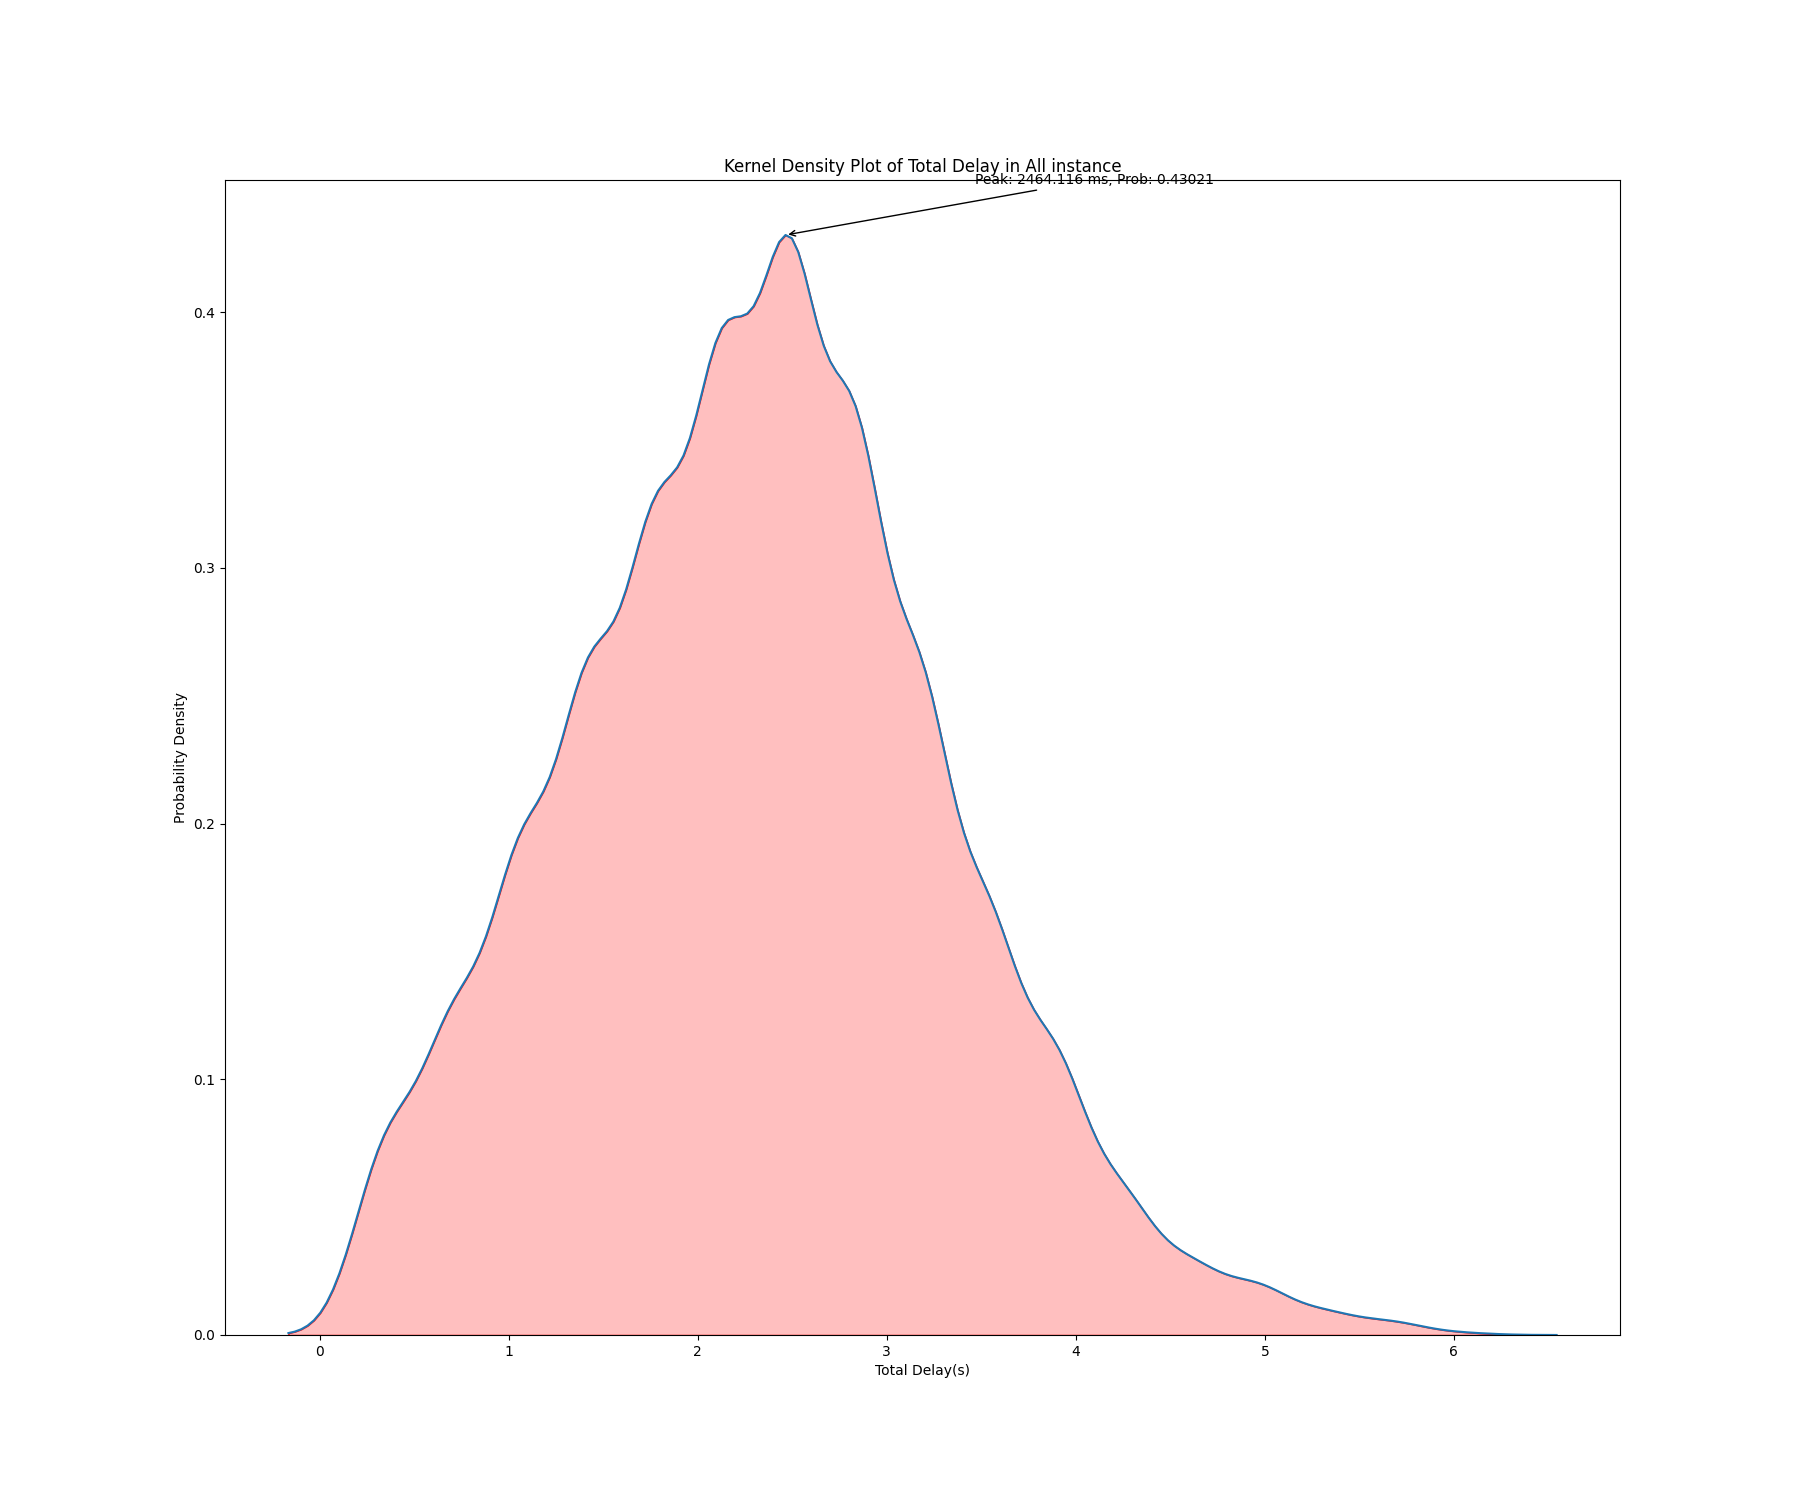
\includegraphics[width=\linewidth]{images/Total Delay density4.png}
        \caption{SF10}
    \end{subfigure}
    \\
    \begin{subfigure}{0.45\linewidth}
        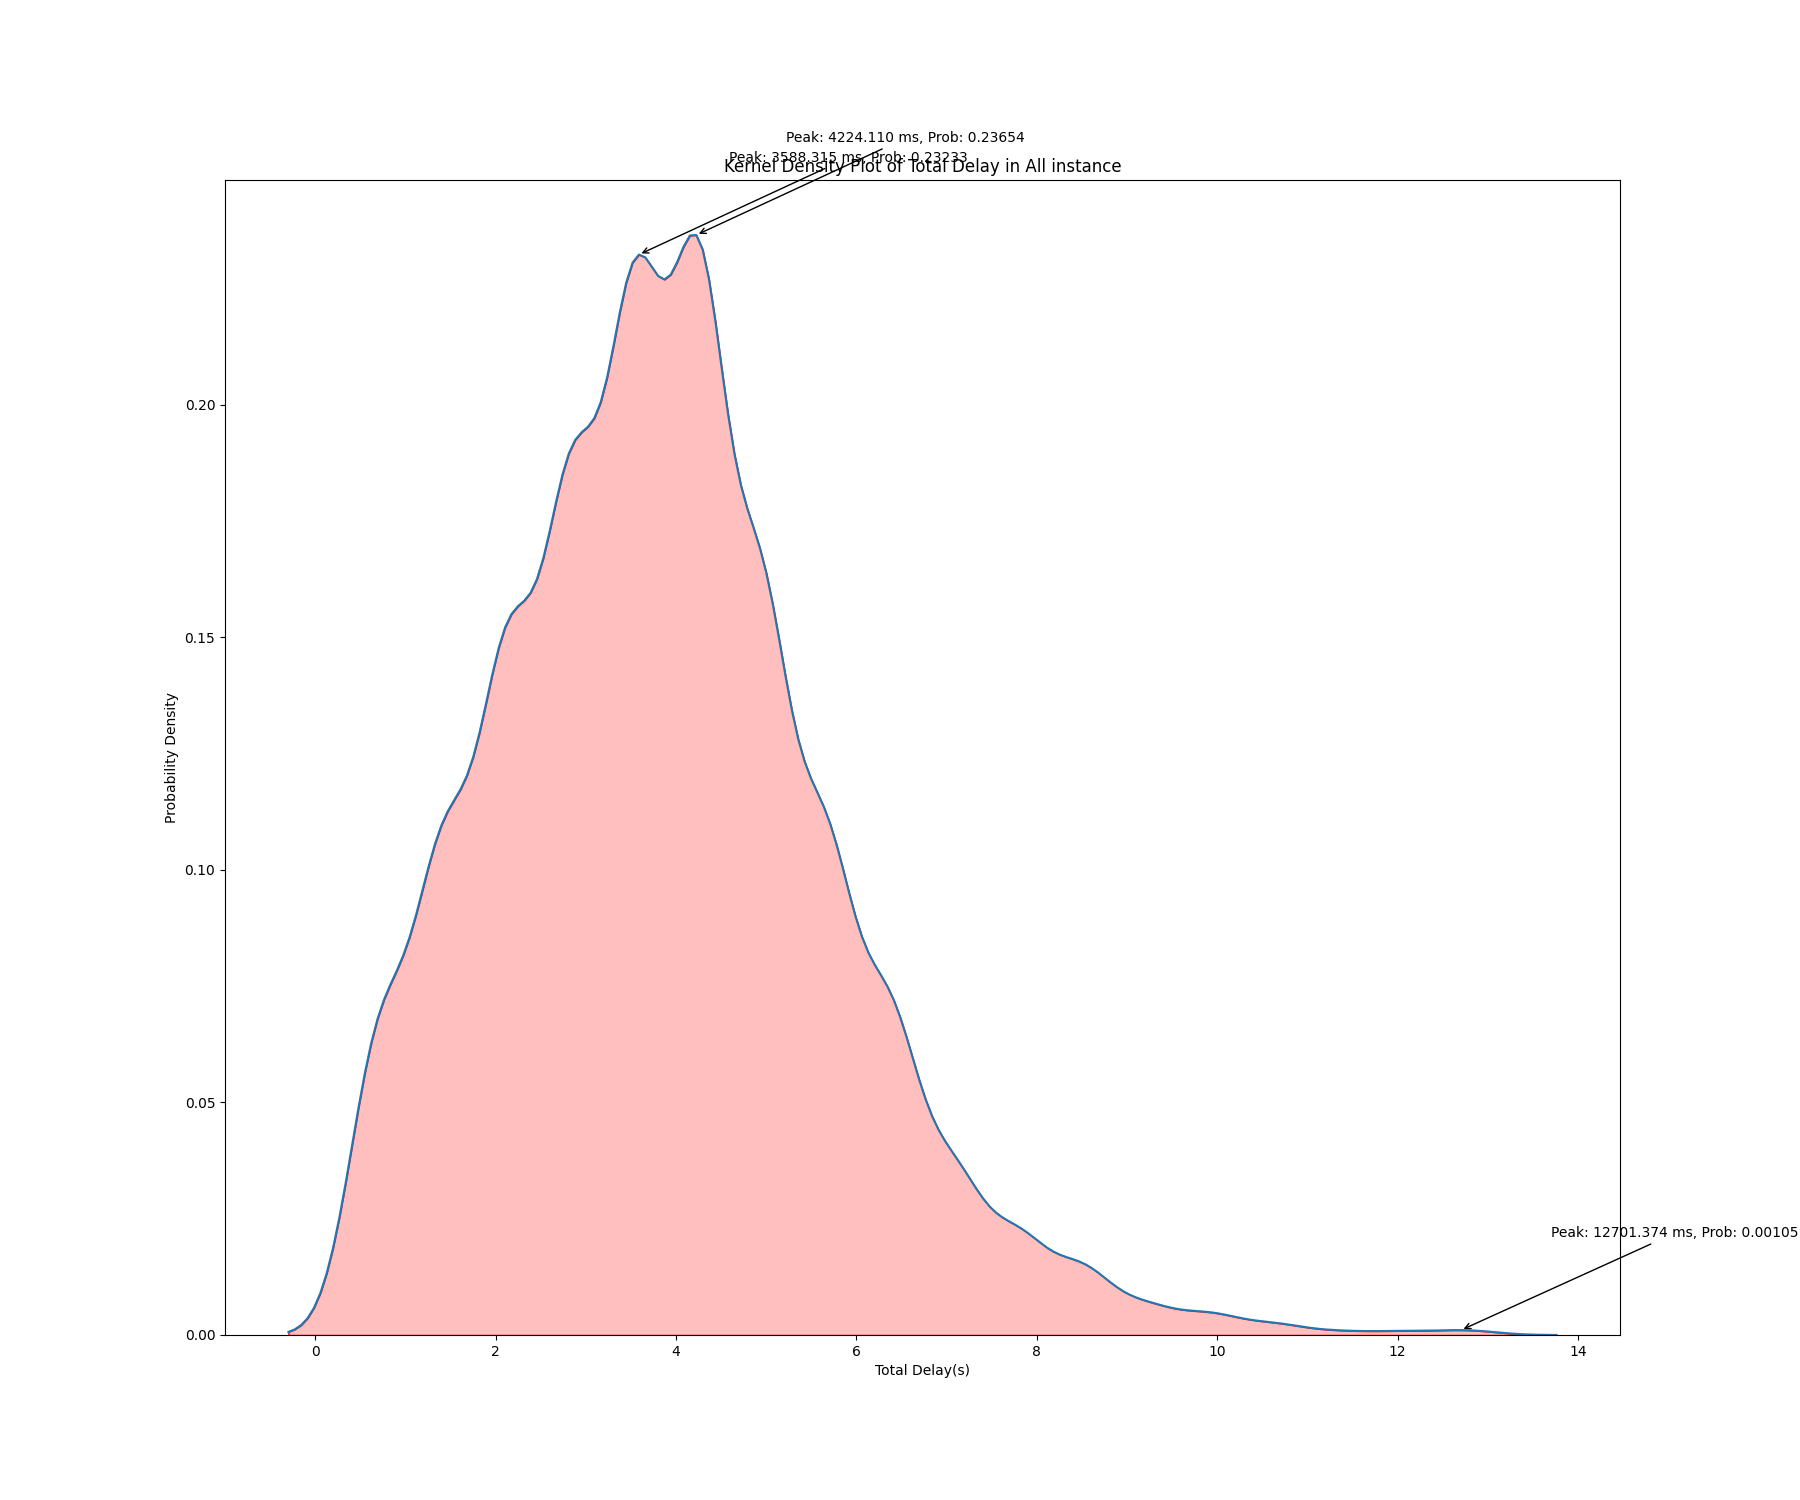
\includegraphics[width=\linewidth]{images/Total Delay density5.png}
        \caption{SF11}
    \end{subfigure}
    \hfill
    \begin{subfigure}{0.45\linewidth}
        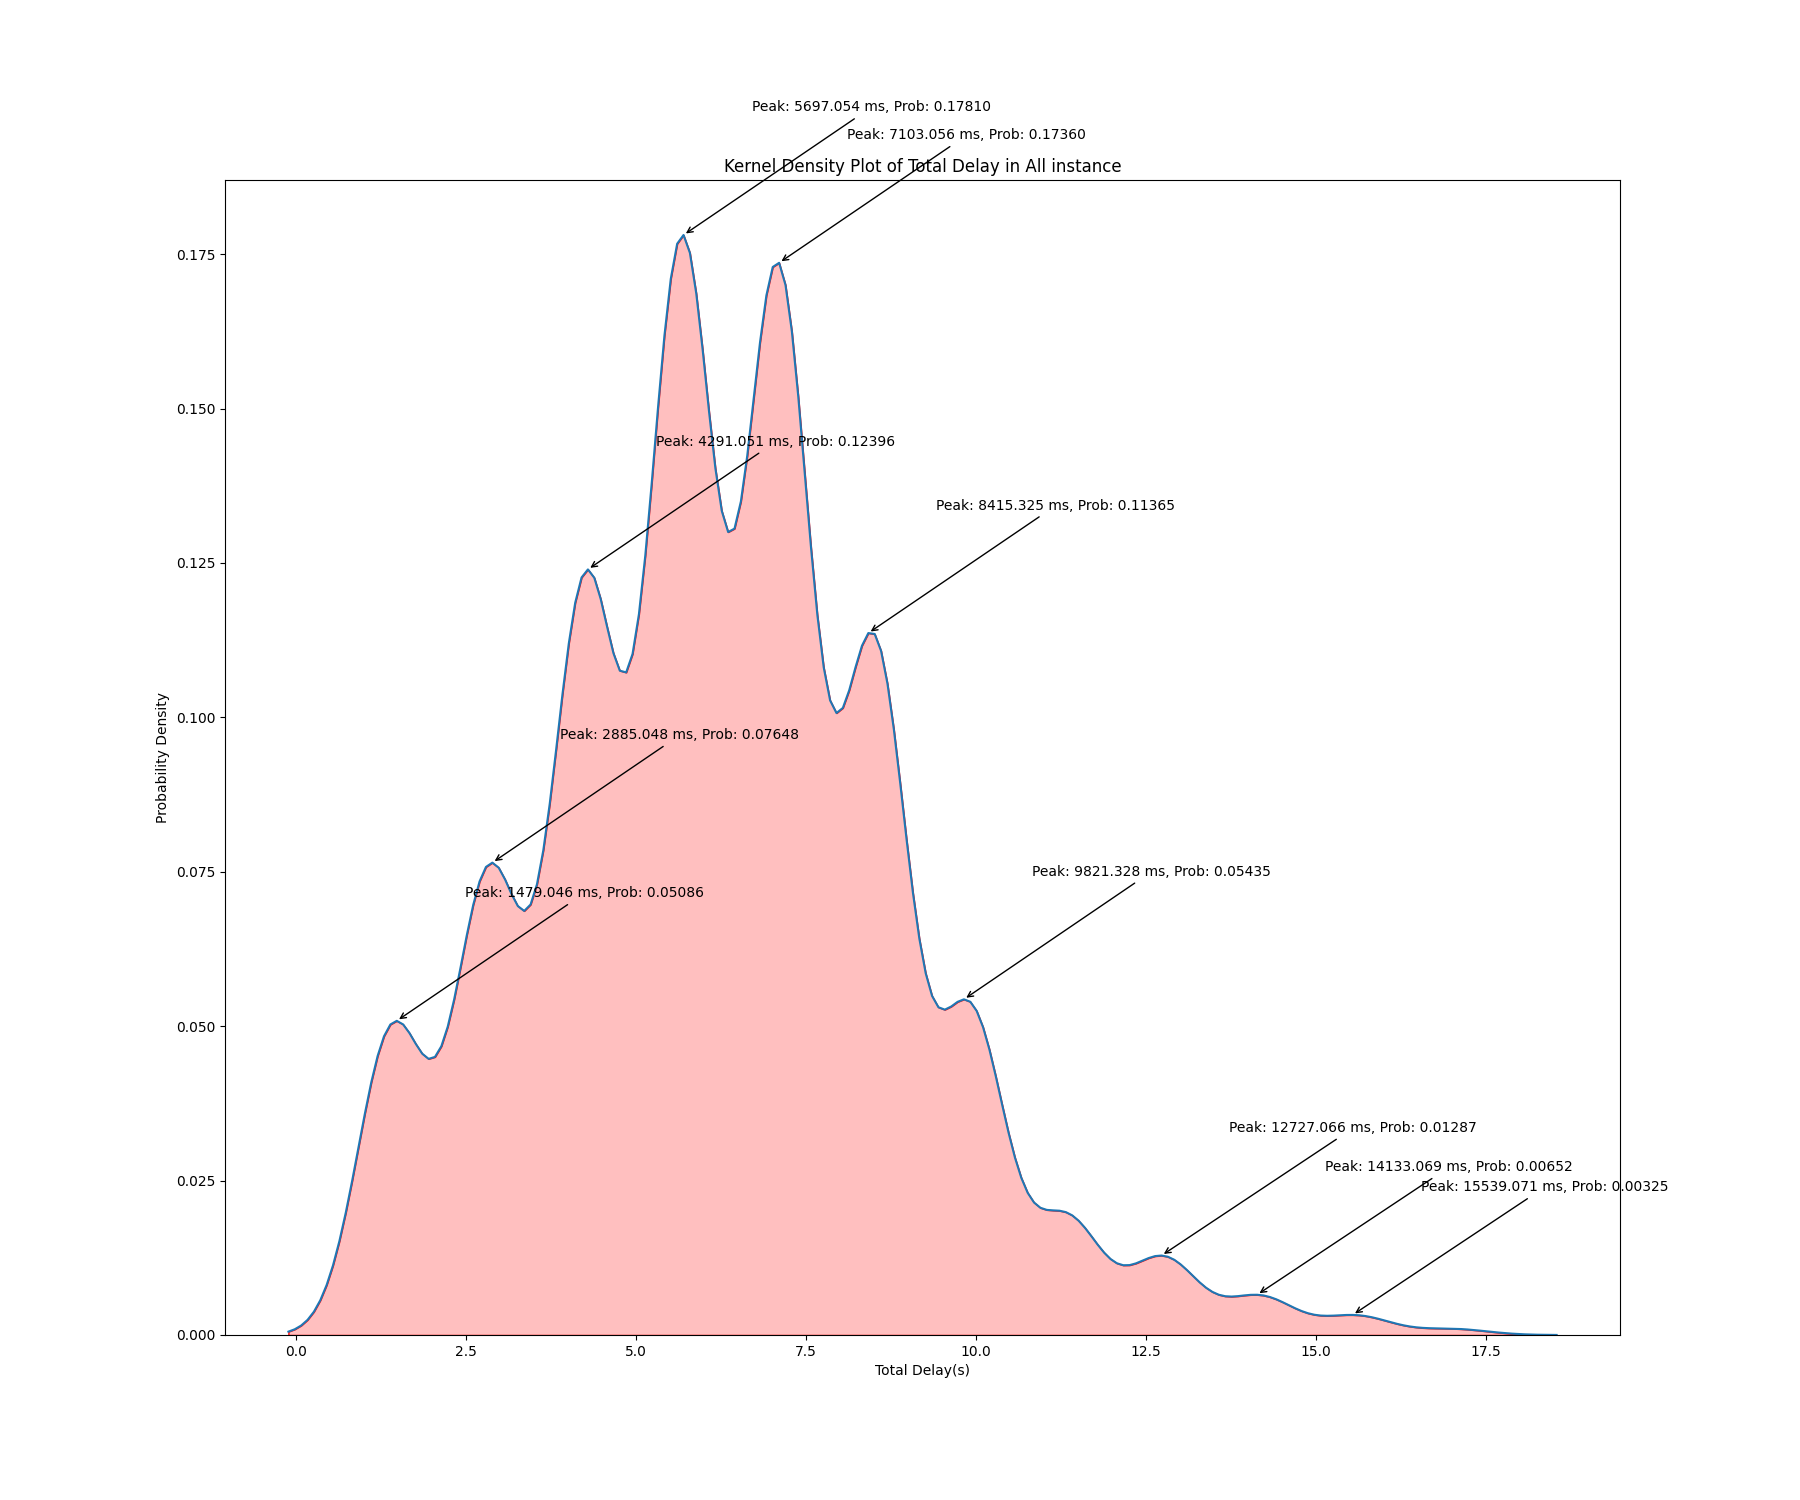
\includegraphics[width=\linewidth]{images/Total Delay density6.png}
        \caption{SF12}
    \end{subfigure}
    \caption{Delay Densities of Spreading Factors}
    \label{fig:density collage}
\end{figure}

\newpage

\begin{figure}[htp!]
    \centering
    \begin{subfigure}{0.45\linewidth}
        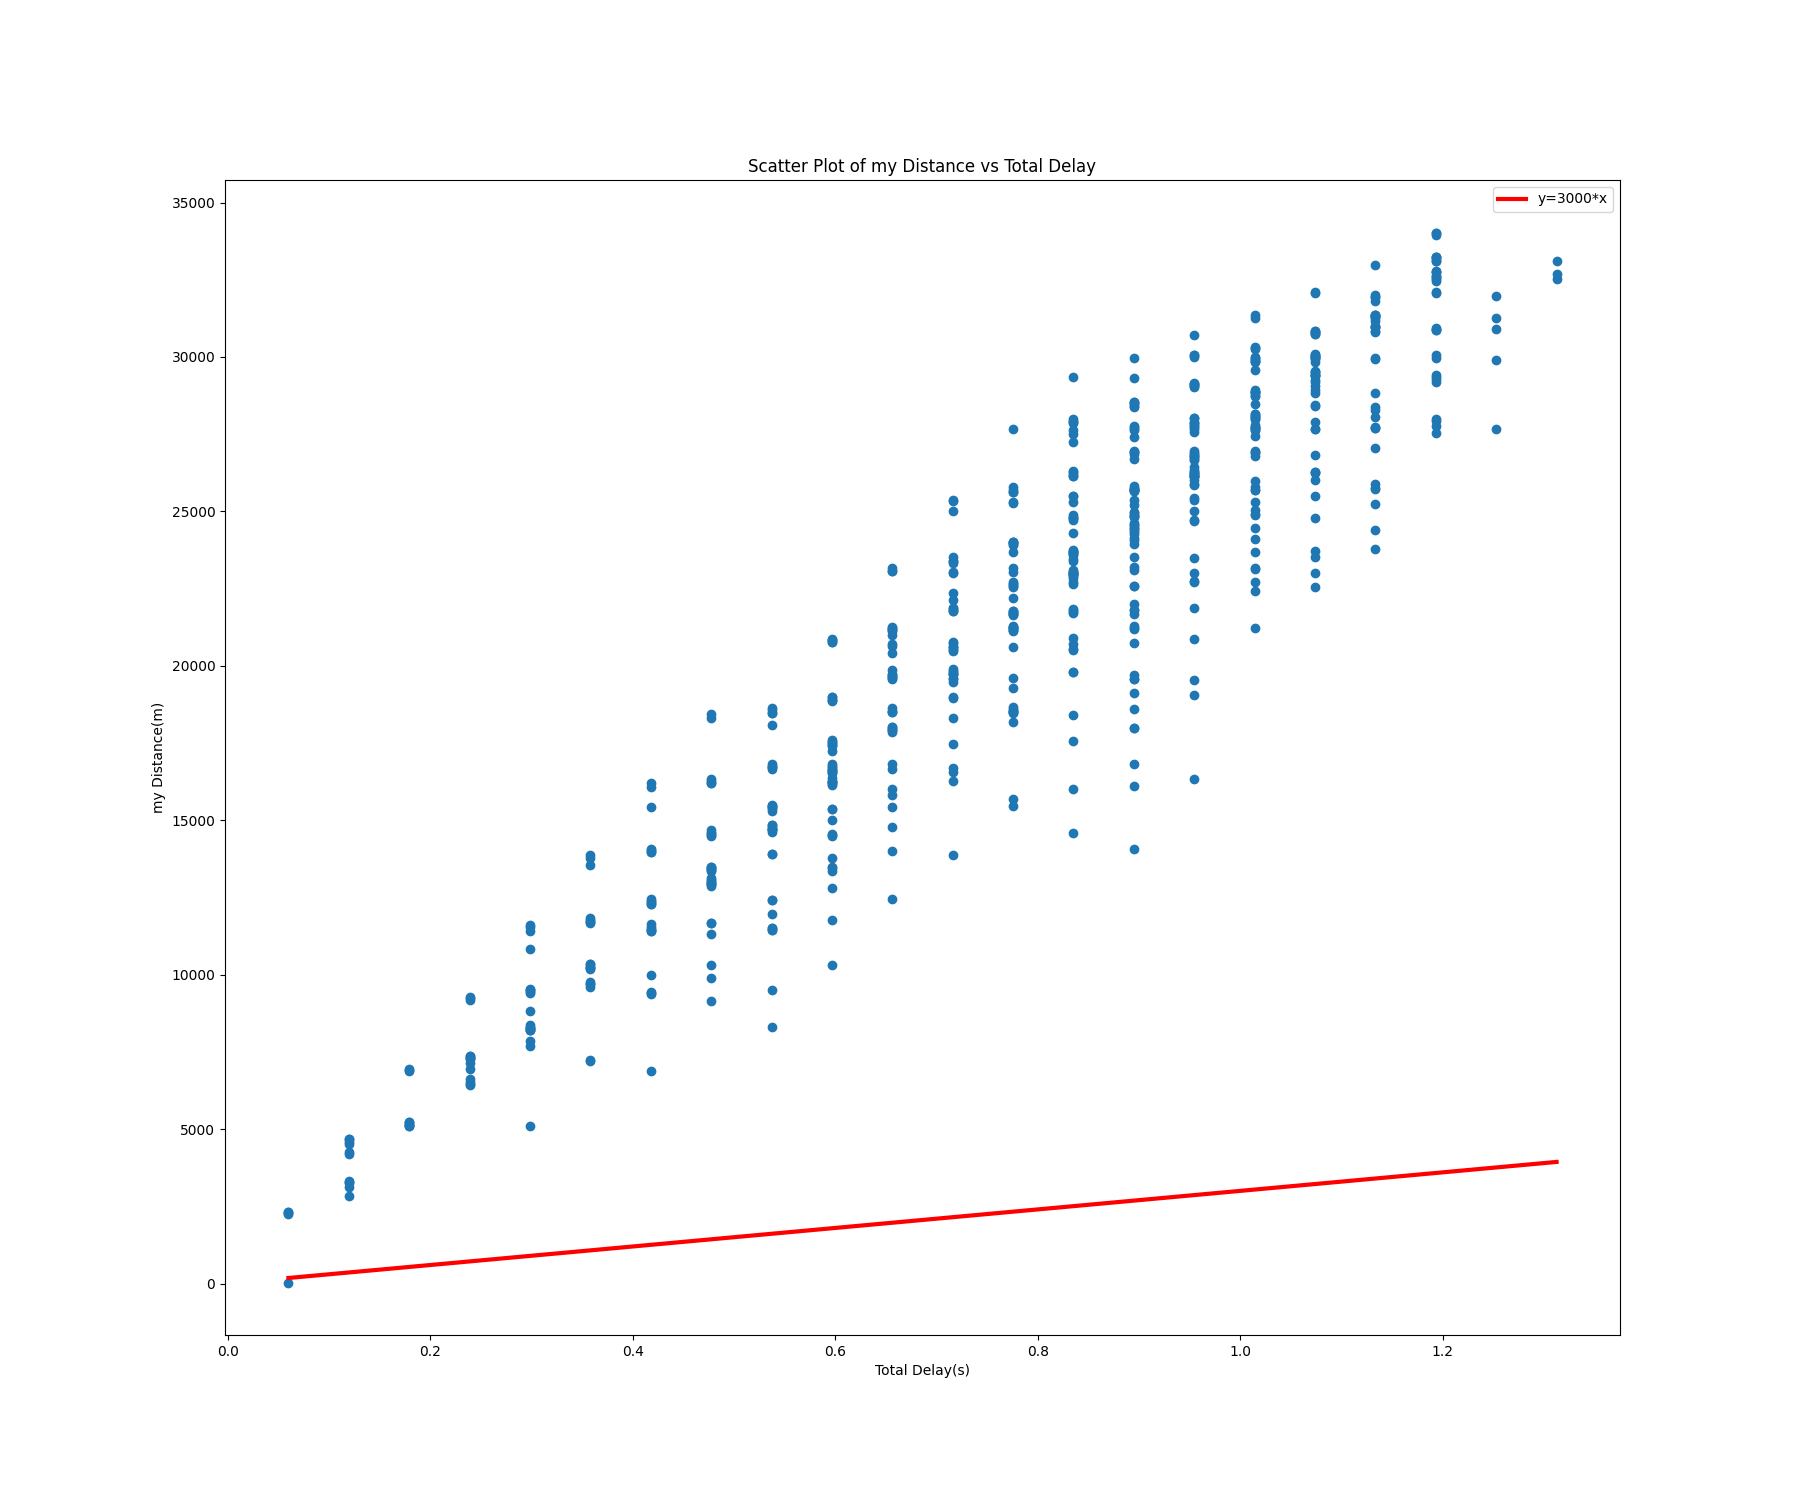
\includegraphics[width=\linewidth]{images/BlindZone1.png}
        \caption{SF7}
    \end{subfigure}
    \hfill
    \begin{subfigure}{0.45\linewidth}
        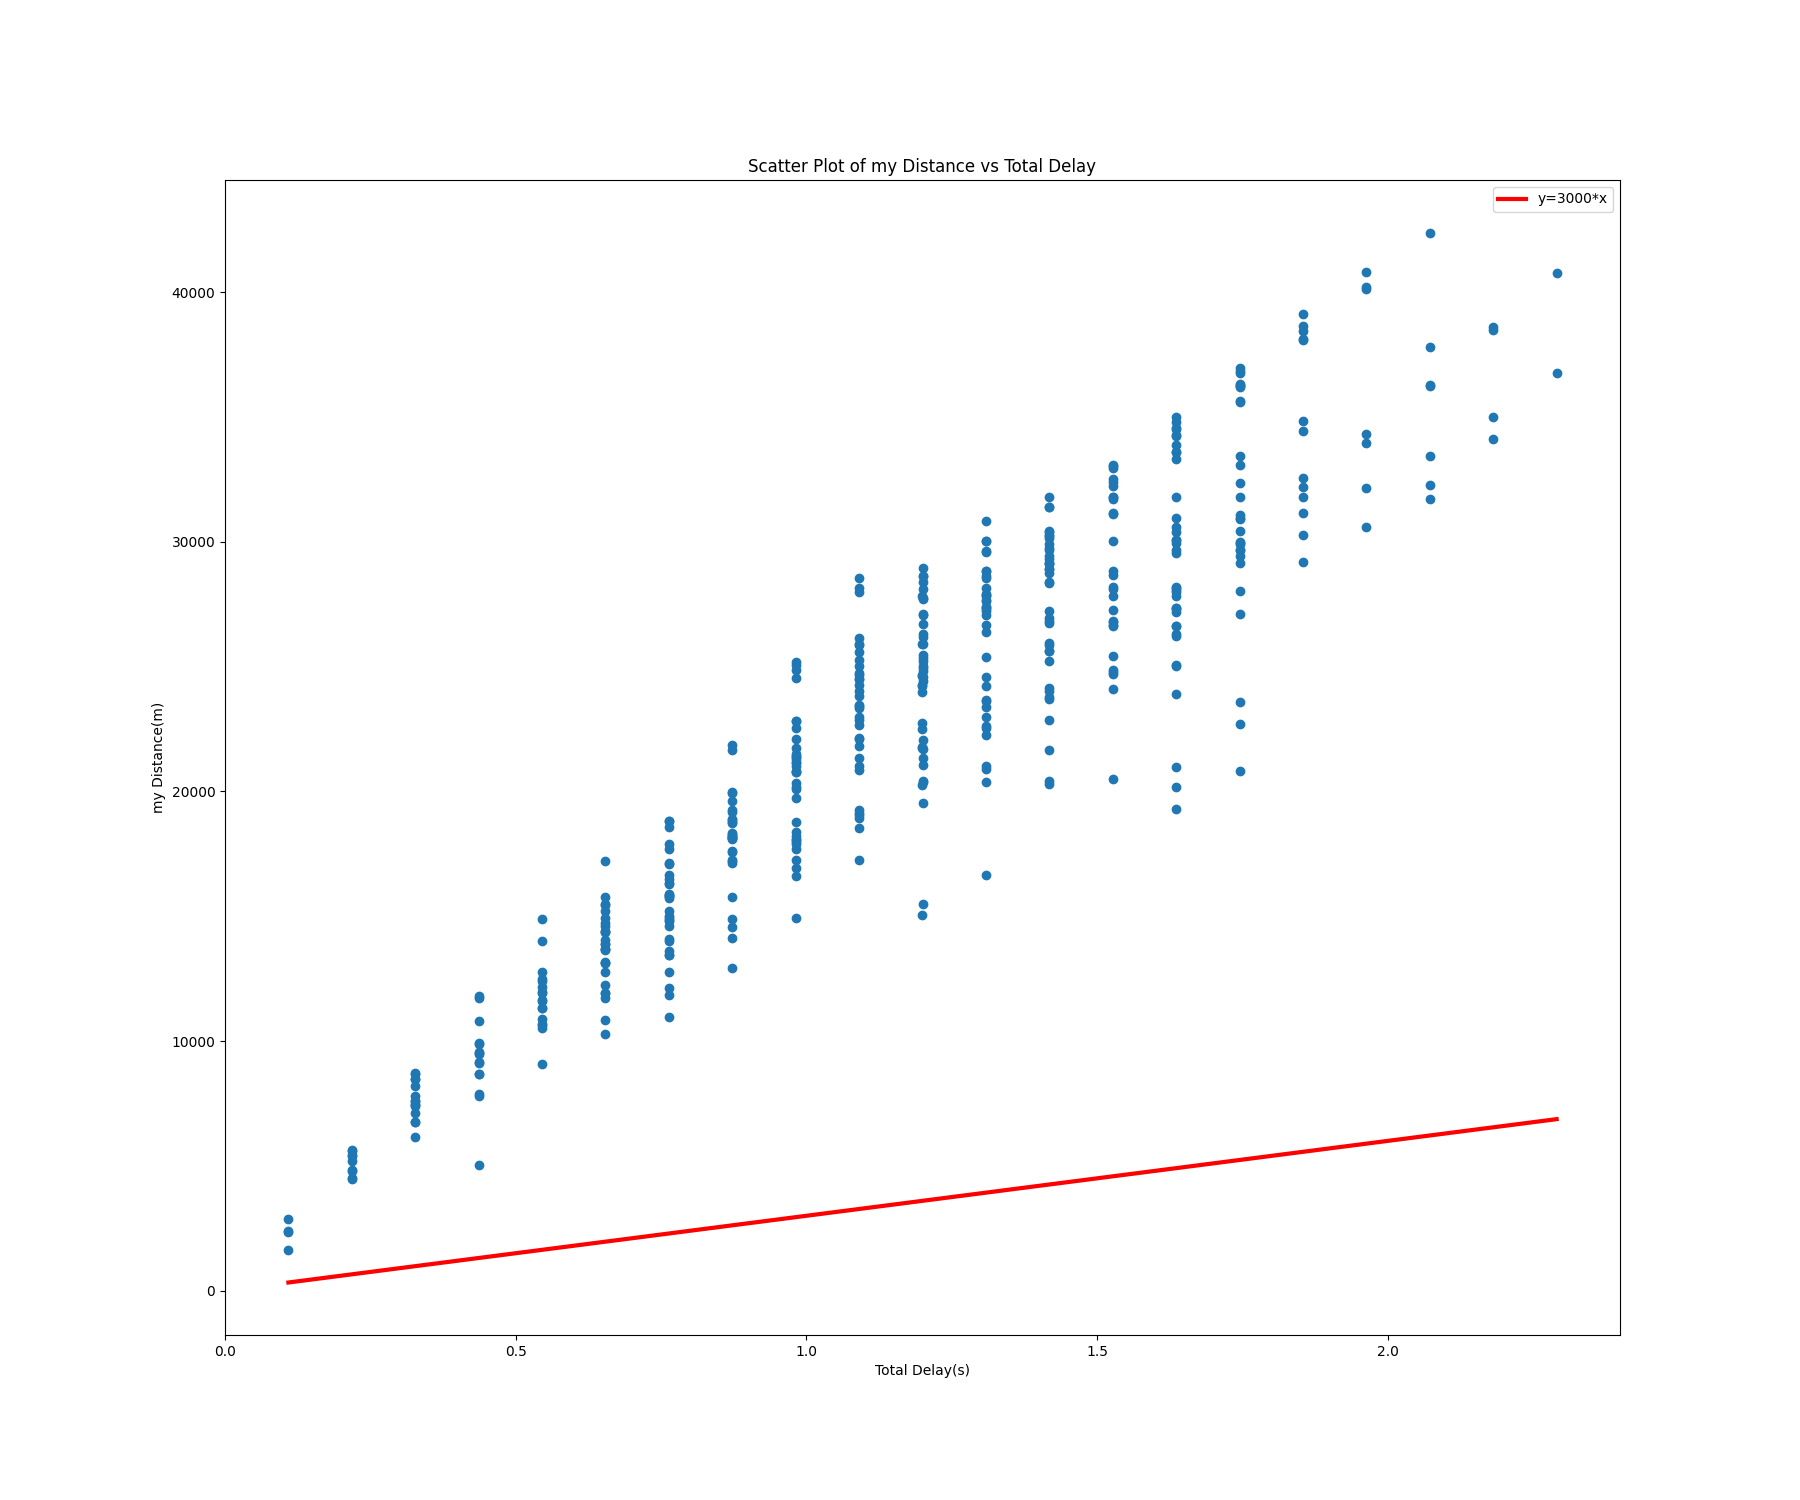
\includegraphics[width=\linewidth]{images/BlindZone2.png}
        \caption{SF8}
    \end{subfigure}
    \\
    \begin{subfigure}{0.45\linewidth}
        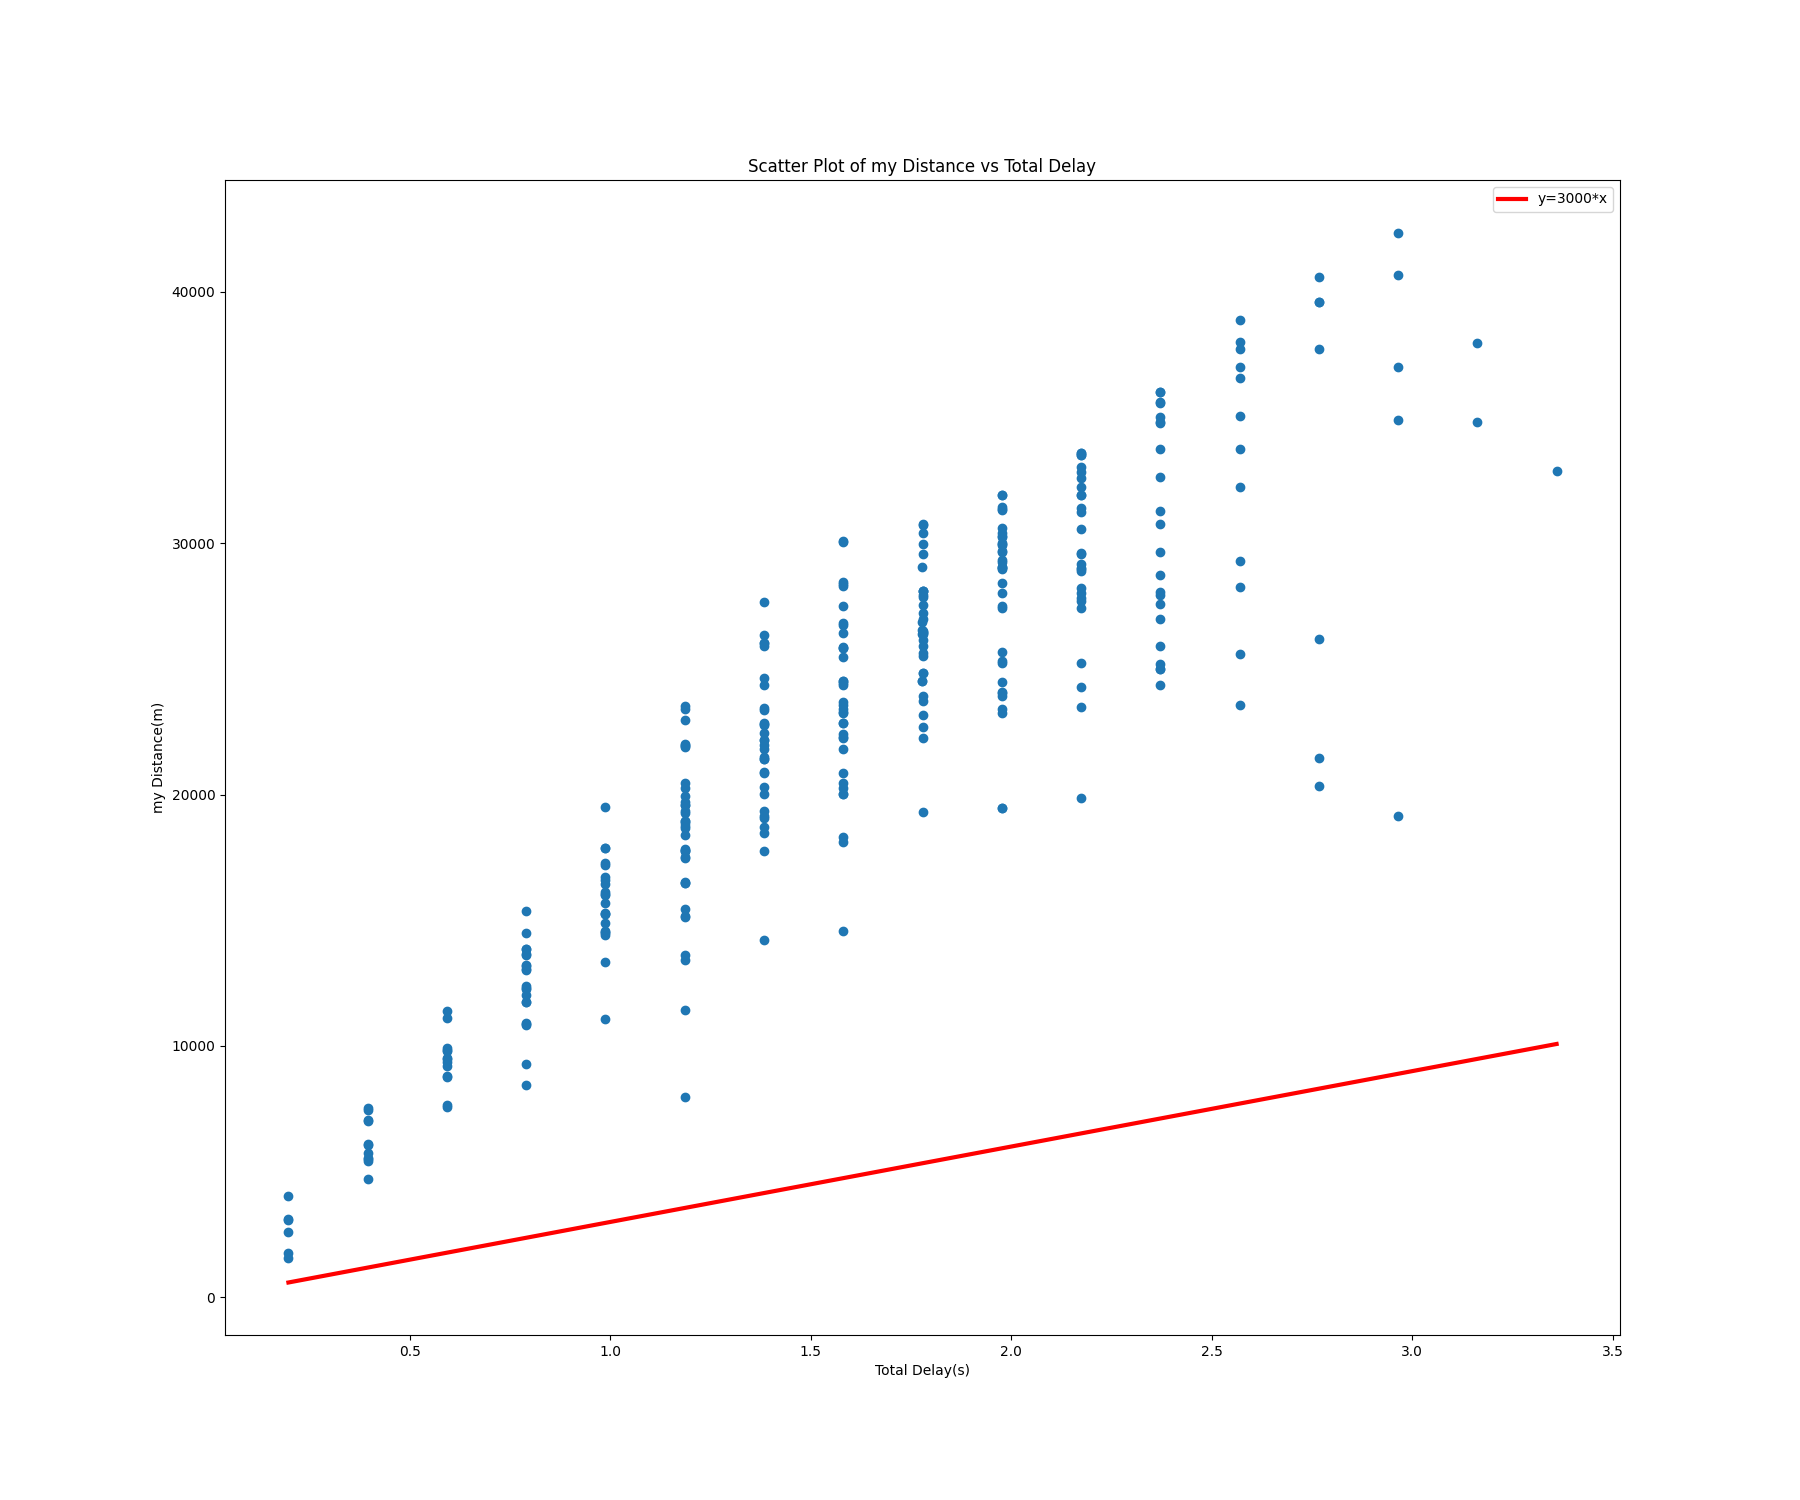
\includegraphics[width=\linewidth]{images/BlindZone3.png}
        \caption{SF9}
    \end{subfigure}
   \hfill
    \begin{subfigure}{0.45\linewidth}
        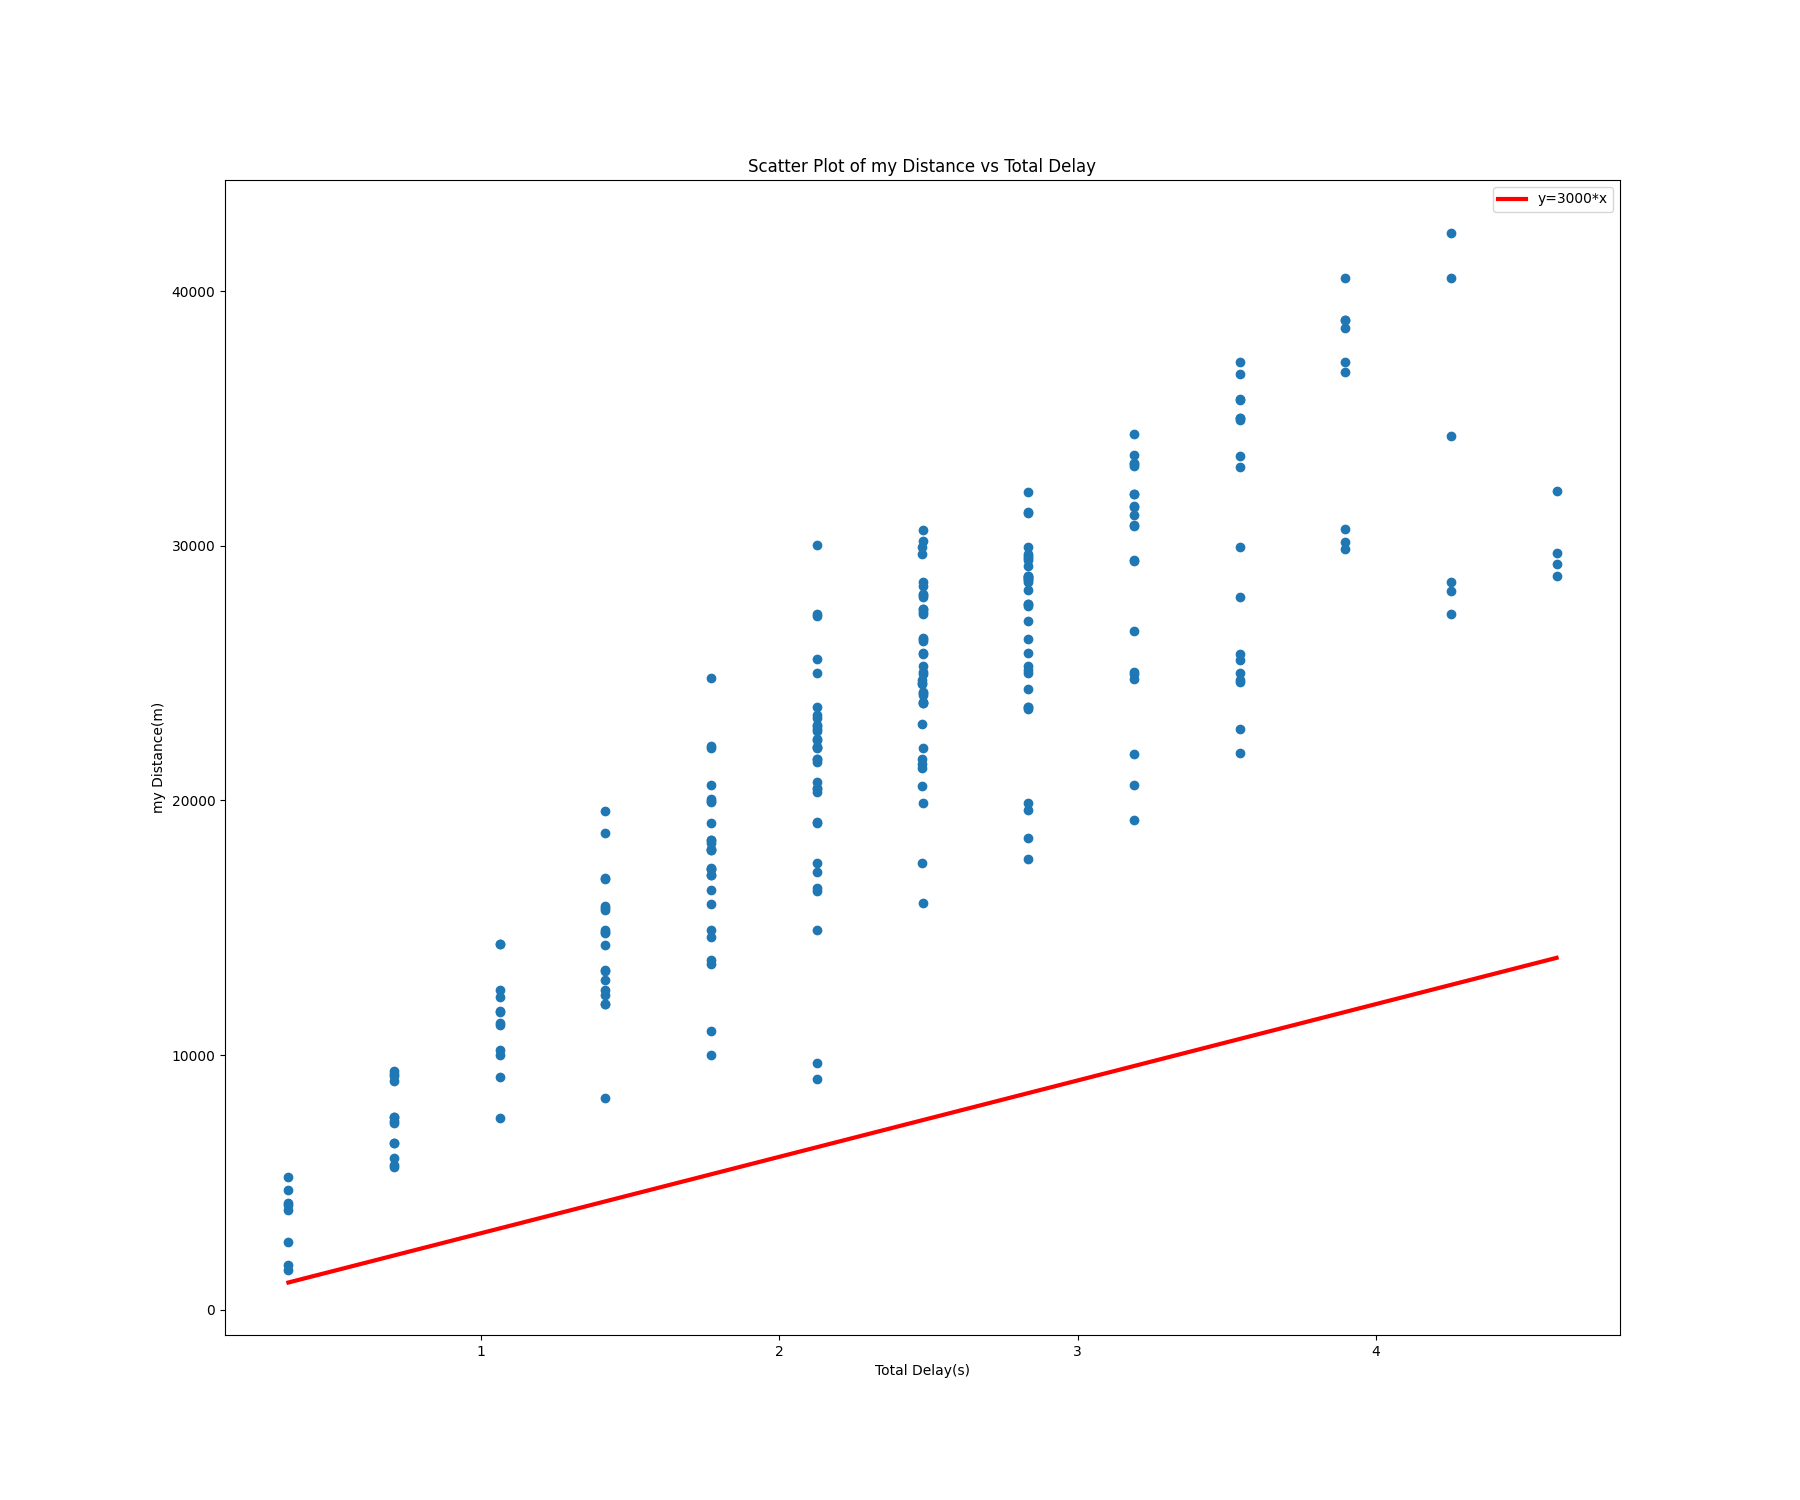
\includegraphics[width=\linewidth]{images/BlindZone4.png}
        \caption{SF10}
    \end{subfigure}
    \\
    \begin{subfigure}{0.45\linewidth}
        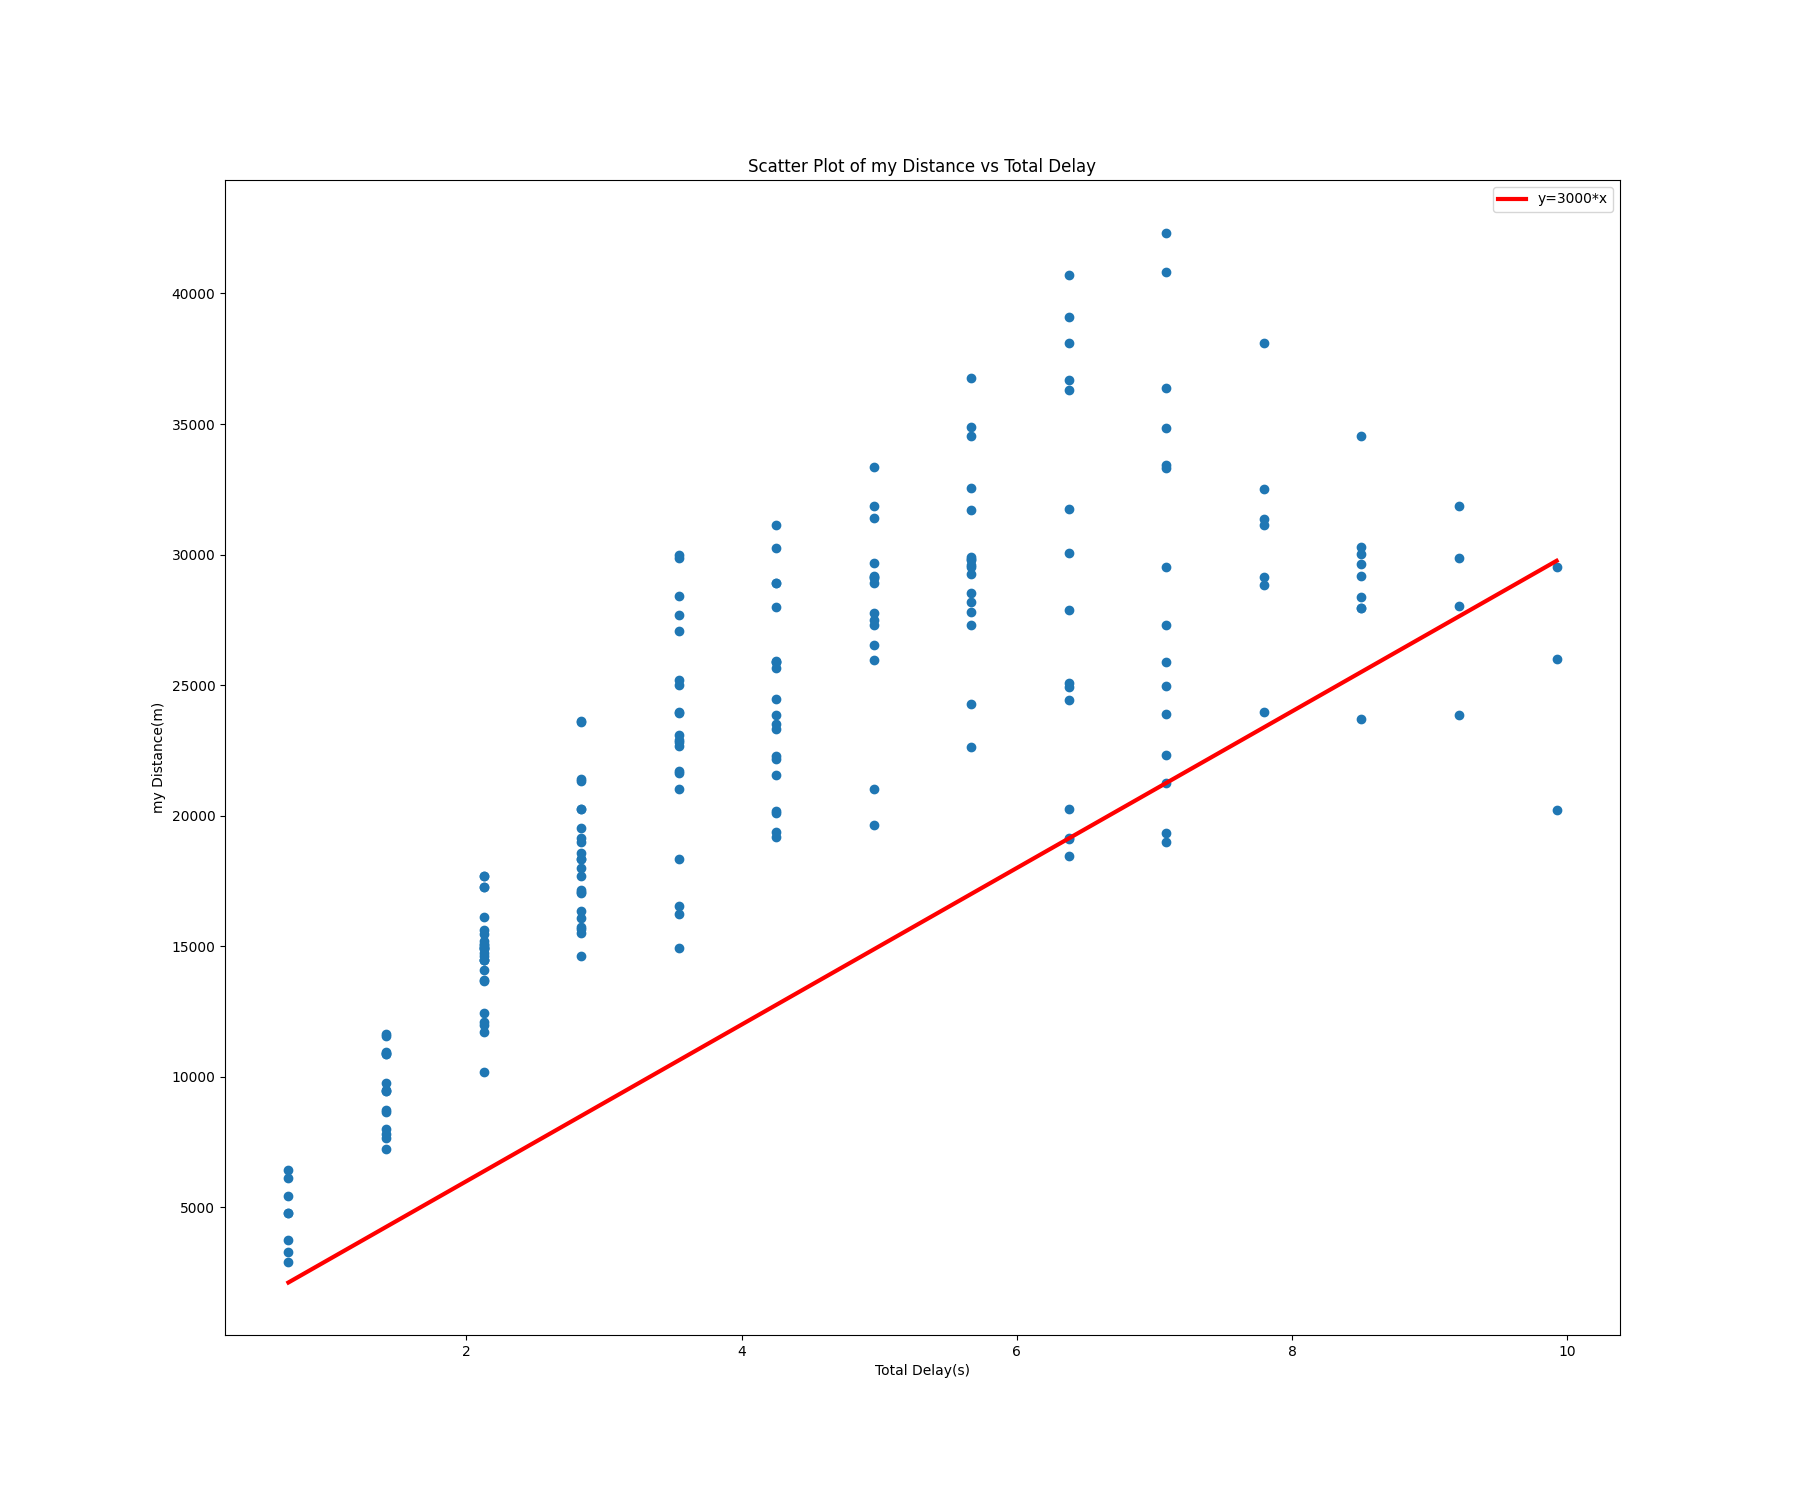
\includegraphics[width=\linewidth]{images/BlindZone5.png}
        \caption{SF11}
    \end{subfigure}
    \hfill
    \begin{subfigure}{0.45\linewidth}
        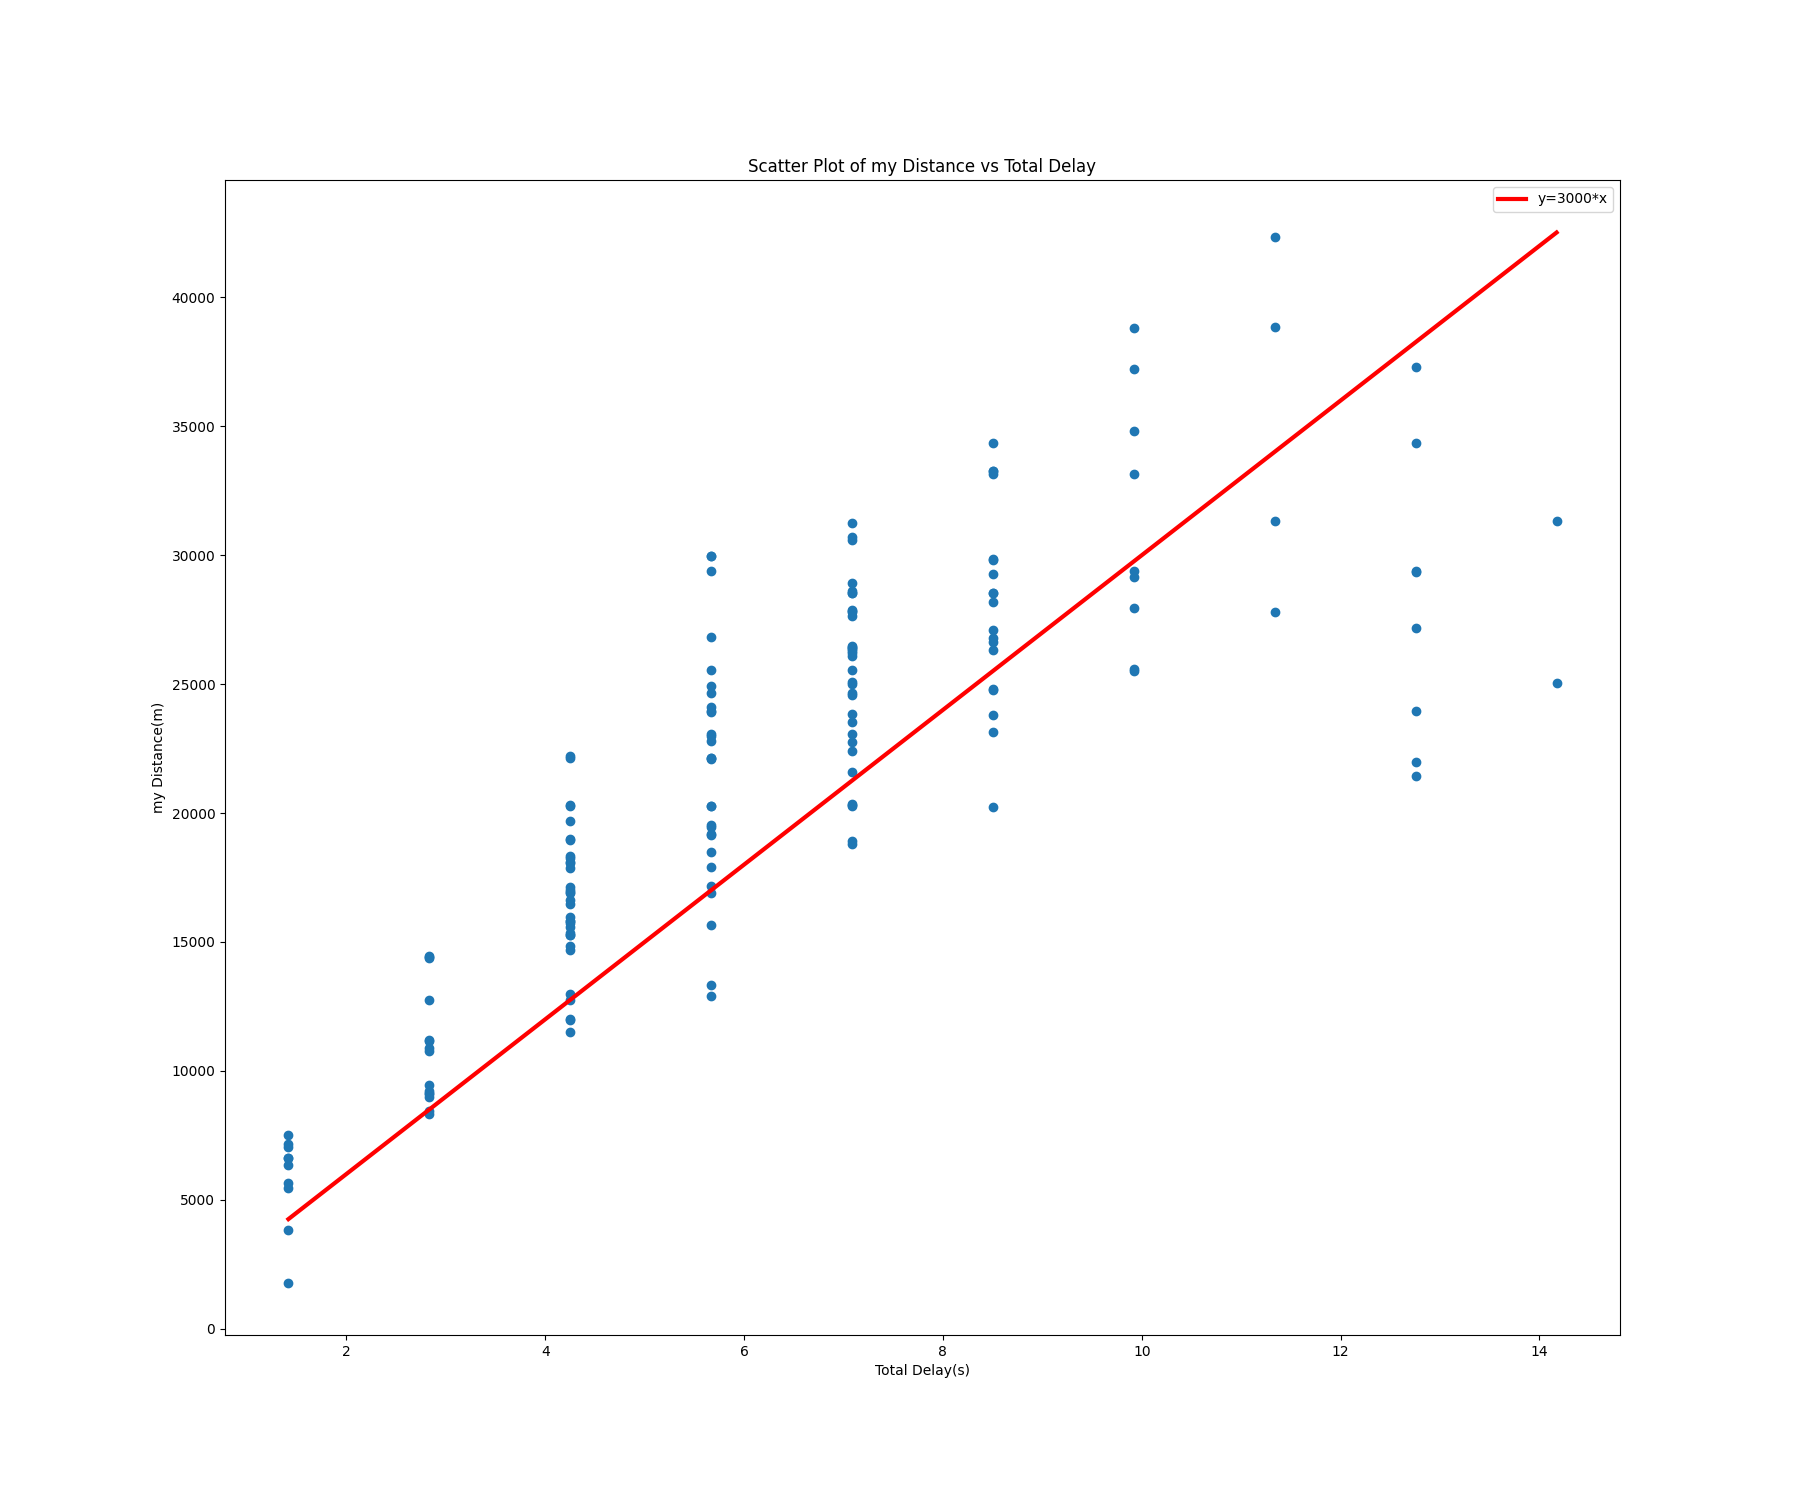
\includegraphics[width=\linewidth]{images/BlindZone6.png}
        \caption{SF12}
    \end{subfigure}
    \caption{Blind zones of Spreading Factors}
    \label{fig:blindzone collage}
\end{figure}

\newpage


We obtain our data from the above \autoref{fig:density collage} to analyze the best spreading factors.


\begin{table}[htp!]
\caption{Results of Spreading Factors}
\small
\setlength{\tabcolsep}{4pt}
\begin{tabular}{|c|c|c|c|c|c|c|}
\hline
\textbf{\begin{tabular}[c]{@{}c@{}}SF\end{tabular}} &
  \textbf{\begin{tabular}[c]{@{}c@{}}Avg \\ unreached\\ End nodes\end{tabular}} &
  \textbf{\begin{tabular}[c]{@{}c@{}}Avg \\ unreached\\ Relay nodes\end{tabular}} &
  \textbf{\begin{tabular}[c]{@{}c@{}}Max time \\ taken to\\ reach Nodes\end{tabular}} &
  \textbf{\begin{tabular}[c]{@{}c@{}}Avg time \\ taken to\\ reach nodes\end{tabular}} &
  \textbf{\begin{tabular}[c]{@{}c@{}}Early Warning \\ Avg time \\ Advantage\end{tabular}} &
  \textbf{\begin{tabular}[c]{@{}c@{}}Avg Hops \\ to reach \\ nodes\end{tabular}} \\ \hline
7  & 0.92\% & 10.05\% & 1.5s  & 0.86s & 8.26s & 14 \\ \hline
8  & 0.00\% & 0.34\%  & 2.5s  & 1.18s & 7.9s  & 11 \\ \hline
9  & 0.00\% & 0.00\%  & 4s    & 1.75s & 7.29s & 9  \\ \hline
10 & 0.00\% & 0.06\%  & 6s    & 2.46s & 6.32s & 7  \\ \hline
11 & 0.04\% & 0.20\%  & 12.5s & 4.22s & 3.81s & 6  \\ \hline
12 & 0.36\% & 0.38\%  & 17.5s & 5.69s & 1.12s & 4  \\ \hline
\end{tabular}
\end{table}

We previously rejected \ac{SF} 7 due to high relay density. Once again, we can dismiss \ac{SF} 7 because the average percentage of unreached relay nodes is 10.05$\%$, indicating a significant packet collision. This observation is evident in the \autoref{fig:nodeplacement collage} graph for \ac{SF} 7, where nodes at the corners of the square area did not receive the packets.

Based on the results presented in the table above, we can recommend \ac{SF} 8 and \ac{SF} 9 as the optimal spreading factor parameters. This recommendation stems from the fact that the average percentages of unreached end and relay nodes are nearly 0$\%$ across 25 iterations for both \ac{SF} 8 and \ac{SF} 9. Additionally, \ac{SF} 8 and \ac{SF} 9 exhibit early warning average times exceeding 7 seconds. 

A crucial consideration is the significantly lower density compared to \ac{SF} 7, given our system's low-cost nature. Hence, this aspect also warrants consideration. When comparing \ac{SF} 10, 11, and 12, it also exhibit lower relay node densities. However, the issue arises with the maximum time taken to reach nodes, which is higher compared to \ac{SF} 8 and \ac{SF} 9. Due to above reasons we can say \ac{SF} 8, \ac{SF} 9 are the most suitable Spreading Factors to our suggest generalized \ac{EEWs} architecture.

\section{Results based on S-wave detection and P-wave detection}\label{ch:results_s_p}

\hspace{12pt} The sensing, detection, and verification aspects are not within our scope, but we have evaluated some results of S-wave and P-wave-based detection. The difference between S-wave and P-wave detection lies in the fact that if we can detect the P-wave, we can gain a time advantage before the S-wave reaches the first earthquake detection point. This advantage stems from the differing ground speeds of P-wave and S-wave, which are approximately $6 km^{-1}$ and $3 km^{-1}$ respectively. Therefore, there is a significant time advantage if an earthquake occurs far away from the initial detection point. However, the problem is that P-waves are body waves, making them very hard to detect. \\

Despite the current system in New Zealand utilizing S-wave detection, in the \autoref{fig:swave detection}, we illustrate the average percentage of nodes versus time available for preparedness if the detection is based on the S-waves.

\newpage

\begin{figure}[ht!]
    \centering
    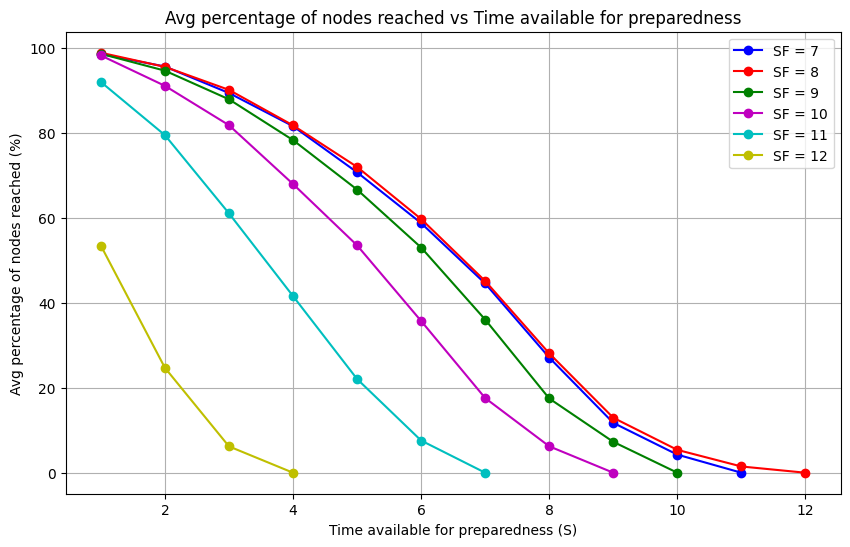
\includegraphics[width=0.8\linewidth]{images/S-wave detection.png}
    \caption{Avg percentage of nodes reached vs Time available for preparedness (S-wave)}
    \label{fig:swave detection}
\end{figure}

The \autoref{fig:pwave detection} illustrates earthquake detection using the P-wave. Here, we assume the earthquake occurred 10km away from the initial detection point. The graph depicts the average percentage of nodes versus the time available for preparedness.


\begin{figure}[ht!]
    \centering
    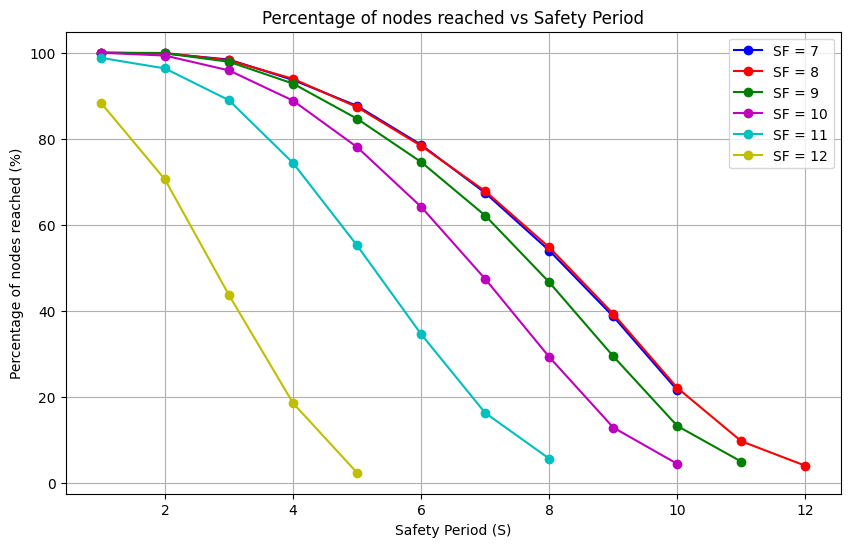
\includegraphics[width=0.8\linewidth]{images/p-wave detection.png}
    \caption{Avg percentage of nodes reached vs Time available for preparedness (P-wave)}
    \label{fig:pwave detection}
\end{figure}

\section{Demostrating Scale-Down Version}\label{ch:scale-down}

\hspace{12pt} Due to the impracticality of testing a system for a 30 km long range in physical testing, we developed a scaled-down test to evaluate and showcase a working emulation of our proposed network architecture. This test utilized a 2dBm transmitting power and was conducted within the university premises. Within the constraints of our device capabilities, we integrated 4 relays and 4 end nodes (1 transmitter and 3 receivers) in our scaled-down scenario. It's important to note that the test environment contained numerous obstacles such as buildings and trees. The node placement for the scaled-down test is depicted in the \autoref{fig:scale-down}.\\

\begin{figure}[ht!]
    \centering
    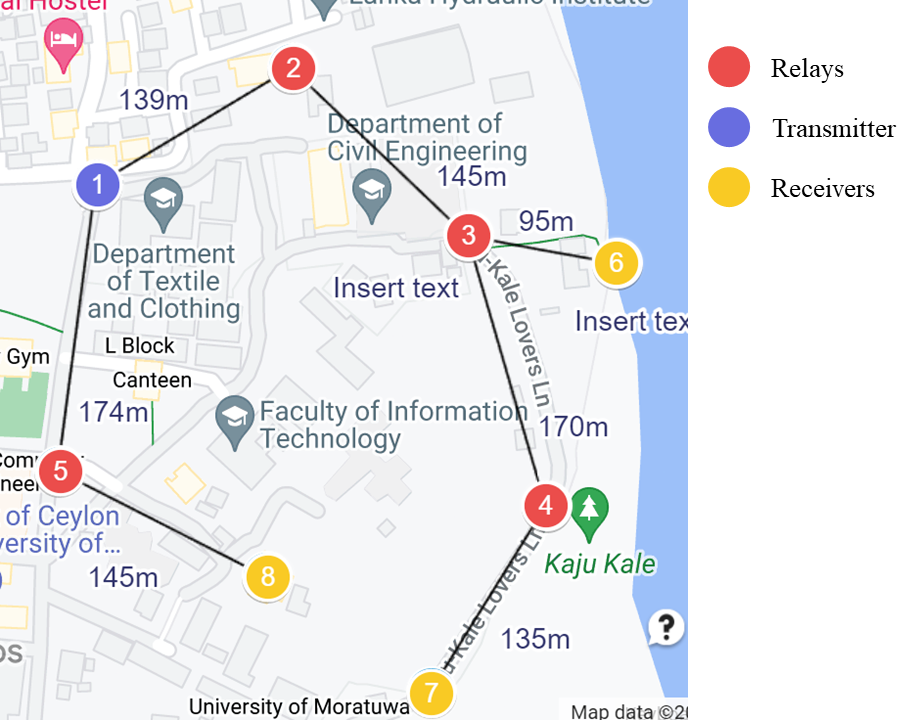
\includegraphics[scale=0.6]{images/scale-down-map.png}
    \caption{Node placement of the scale-down experiment}
    \label{fig:scale-down}
\end{figure}

In our proposed communication setup, both the transmitter and relays broadcast messages to multiple devices. We aimed to replicate this feature in our scaled-down scenario. Specifically, Node 1 transmits messages to both Node 2 and Node 3, while Node 3 transmits messages to both Node 6 and Node 4. On the other hand, in the real architecture, a single node may receive warning messages from multiple devices. In our scaled-down test, Node 6 receives messages from both Node 3 and Node 4.\\

\noindent \textbf{Scaling Up Scaled-Down Tests to Simulate Real-World Conditions}\\

The primary motivation behind conducting a scaled-down test was to address the challenge of achieving greater distances in practical scenarios. Despite using a 2dBm transmitting power for our scaled-down tests, in our real communication setup, we employ a transmitting power of 17dBm. Therefore, we analyzed how the scaled-down test could be scaled up to accommodate higher transmitting power. In this process, the receiving power at the receiver of the scaled-down scenario equals that of the receiver in the scaled-up scenario.\\
\\
The receiving power can be determined using the following equation.
\begin{equation}
    P_{Rx} = P_{Tx} + G_{Rx} + G_{Tx} - PL 
\end{equation}
$P_{Rx}$: Receiving power\\
$P_{Tx}$: Transmitting power\\
$G_{Rx}$: Receiving antenna gain\\
$G_{Rx}$: Transmitting antenna gain\\
$PL$: Path loss (Taking from the Log Normal Shadowing model)\\

\noindent Calculating the receiving power in the scaled-down scenario,
\begin{equation}
    P_{Rx\_sd} = P_{Tx\_sd} + G_{Rx} + G_{Tx} - (PL(d_{0}) + 10 \: \gamma \: log_{10}(d_{sd}/d_{0}) + X_{\sigma})
\end{equation}

\noindent Calculating the receiving power in the scaled-down scenario,
\begin{equation}
    P_{Rx\_su} = P_{Tx\_su} + G_{Rx} + G_{Tx} - (PL(d_{0}) + 10 \: \gamma \: log_{10}(d_{su}/d_{0}) + X_{\sigma})
\end{equation}

Since \( P_{\text{Rx\_sd}} \) and \( P_{\text{Rx\_su}} \) are the same, as mentioned above, and since we scale up the same link in the scaled-down version, we believe the shadowing effect remains unchanged. Therefore, we assume that the impact of \( X_{\sigma} \) is consistent in both scenarios.\\

\noindent Then we obtain:
\begin{equation}
    P_{Tx\_sd} - 10 \: \gamma \: log_{10}(d_{sd}) \approx P_{Tx\_su} - 10 \: \gamma \: log_{10}(d_{su})
\end{equation}
\begin{equation}
    10 \: \gamma \: log_{10}(d_{su}) - 10 \: \gamma \: log_{10}(d_{sd}) \approx P_{Tx\_su} - P_{Tx\_sd}
\end{equation}
\begin{equation}
    10 \: \gamma \: log_{10}(d_{su}/d_{sd}) \approx P_{Tx\_su} - P_{Tx\_sd}
\end{equation}
\begin{equation}
    (d_{su}/d_{sd}) \approx 10 ^ {\frac{P_{Tx\_su} - P_{Tx\_sd}}{10 \: \gamma}}
    \label{eq:ratio}
\end{equation}
\hspace{12pt} Therefore, by \autoref{eq:ratio}, we can determine the ratio between the scaled-up distance and the scaled-down distance. It's worth mentioning that small variations in the values obtained from this equation compared to the real values may occur. These discrepancies can arise due to factors such as shadowing and other environmental influences.\\

From the \autoref{eq:ratio}, we observe that the scaling-up process may be influenced by the parameter \( \gamma \) of the Log Normal Shadowing model, indicating the impact of environmental factors. Given that our actual system utilizes a 17 dBm transmission power, \autoref{fig:ratio_gamma} illustrates how the ratio between scaled-down distance and scaled-up distance varies with \( \gamma \).
\begin{figure}
    \centering
    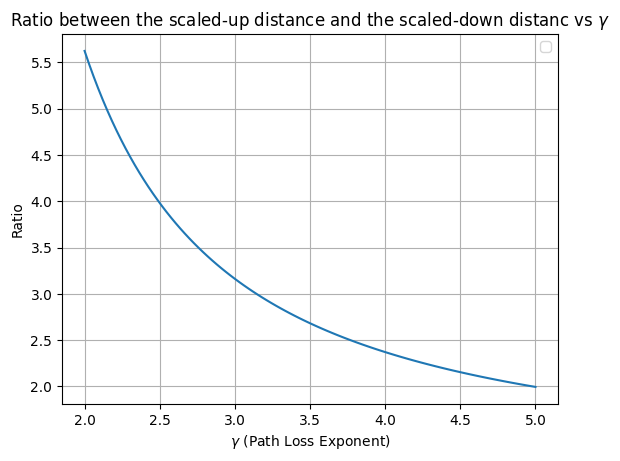
\includegraphics[width=0.8\linewidth]{images/ratio_vs_gamma.png}
    \caption{Variation of the ratio between scale-up and scale-down distance with $\gamma$ (Transmitting power = 17dBm)}
    \label{fig:ratio_gamma}
\end{figure}

\autoref{fig:ratio_power} illustrates how the ratio between scaled-up distance and scaled-down distance varies with the transmitting power for $\gamma = 3.3$.\\
\begin{figure}
    \centering
    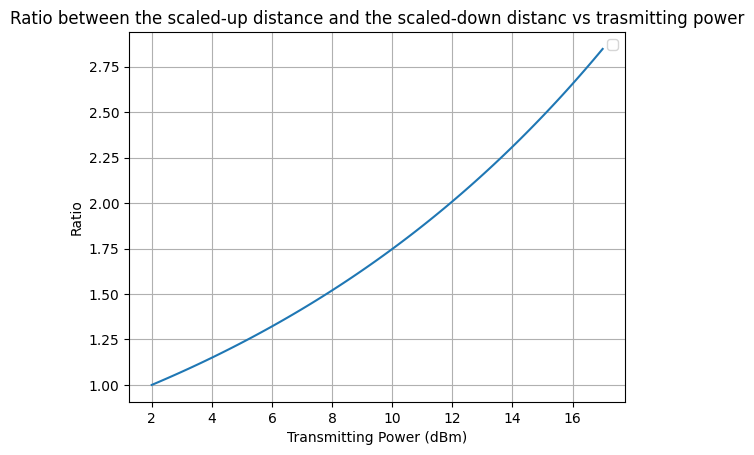
\includegraphics[width=0.8\linewidth]{images/power_ration.png}
    \caption{Variation of the ratio between scale-up and scale-down distance with transmitting power($\gamma = 3.3$)}
    \label{fig:ratio_power}
\end{figure}

\autoref{tab:scale-down-tab} illustrates how our scaled-down experiment can be extrapolated to a scaled-up version of transmitting power of 17 dBm. It's important to note that due to space constraints, we have not maintained the maximum range between the devices. For the calculation, \( \gamma \) is taken as 3.3, which is the value obtained from fine-tuning the parameters of the Log Normal Shadowing model.

\begin{table}[htp!]
\begin{tabular}{|c|c|c|}
\hline
\textbf{Link} &
  \textbf{\begin{tabular}[c]{@{}c@{}}Scaled-down Link \\ Distance in meters (2 dBm)\end{tabular}} &
  \textbf{\begin{tabular}[c]{@{}c@{}}Scaled-up Link \\ Distance in meters (17 dBm)\end{tabular}} \\ \hline
1-2                                                             & 139  & 395.87 \\ \hline
2-3                                                             & 145  & 412.96 \\ \hline
3-4                                                             & 170  & 484.16 \\ \hline
1-5                                                             & 174  & 495.55 \\ \hline
5-8                                                             & 145  & 412.96 \\ \hline
3-6                                                             & 95   & 270.56 \\ \hline
4-7                                                             & 135  & 384.48 \\ \hline
\begin{tabular}[c]{@{}c@{}}Maximum Link\\ Distance\end{tabular} & 1800 & 5126   \\ \hline
\end{tabular}
\caption{Comparison the distances between scale-down (2 dBm) and scale-up (17 dBm) scenarios}
\label{tab:scale-down-tab}
\end{table}
%------------------------------------------------------------------------------------------
